% ═══════════════════════════════════════════════════════════════════════
%  MSE 433 — Final Project Report (LaTeX)
%  Adriel De Vera | April 2026
% ═══════════════════════════════════════════════════════════════════════
\documentclass[11pt,letterpaper]{article}

% ── packages ──────────────────────────────────────────────────────────
\usepackage[margin=1in]{geometry}
\usepackage{graphicx}
\usepackage{booktabs}
\usepackage{amsmath,amssymb}
\usepackage{hyperref}
\usepackage{caption}
\usepackage{subcaption}
\usepackage{float}
\usepackage{enumitem}
\usepackage{xcolor}
\usepackage{fancyhdr}
\usepackage{titlesec}
\usepackage{array}
\usepackage[numbers]{natbib}
\usepackage{parskip}
\usepackage{listings}

\hypersetup{
    colorlinks=true,
    linkcolor=blue!70!black,
    citecolor=blue!70!black,
    urlcolor=blue!70!black,
}

% ── formatting ────────────────────────────────────────────────────────
\pagestyle{fancy}
\fancyhf{}
\fancyhead[L]{\small MSE 433 - Final Project Report}
\fancyhead[R]{\small Adriel De Vera}
\fancyfoot[C]{\thepage}
\renewcommand{\headrulewidth}{0.4pt}

\titleformat{\section}{\large\bfseries}{\thesection}{1em}{}
\titleformat{\subsection}{\normalsize\bfseries}{\thesubsection}{1em}{}
\titlespacing*{\section}{0pt}{1.2em}{0.4em}
\titlespacing*{\subsection}{0pt}{0.8em}{0.2em}

\graphicspath{{../../outputs/}}
\tolerance=1000
\emergencystretch=1em

\lstset{
    basicstyle=\small\ttfamily,
    backgroundcolor=\color{gray!8},
    frame=single,
    framerule=0.4pt,
    rulecolor=\color{gray!40},
    breaklines=true,
    columns=fullflexible,
}

% ══════════════════════════════════════════════════════════════════════
\begin{document}

% ── Compact Title ─────────────────────────────────────────────────────
\begin{center}
{\LARGE\bfseries Optimizing Warehouse Inventory Through\\[4pt]
Demand Forecasting and Stochastic Reorder Policies\par}
\vspace{8pt}
{\large MSE 433 - Final Project Report}\\[4pt]
{\normalsize Adriel De Vera - April 2026}\\[2pt]
\href{https://github.com/AdrielDeVera/mse-433-final}{Github Repository}
\end{center}
\vspace{0.3em}
\hrule
\vspace{1em}


% ══════════════════════════════════════════════════════════════════════
\section{Introduction}
\label{sec:intro}

Warehouse inventory management seems like a simple problem: hold enough stock to meet demand, but not so much that capital is wasted on goods sitting idle. In practice, the difficulty lies in what ``enough'' means across thousands of SKUs with different demand rates, variability profiles, and supplier lead times. When each tier of a supply chain responds to demand noise by ordering a little extra, those small buffers compound upstream - a phenomenon known as the \textbf{bullwhip effect}~\cite{lee1997bullwhip}. The result is simultaneous overstocking in some SKUs and stockouts in others.

The primary stakeholder is a \textbf{warehouse manager} responsible for a mixed-category facility (Pharmaceuticals, Automotive, Electronics, Groceries, Apparel) who currently applies a single, globally parameterised static reorder rule: a fixed number of days of historical average demand as safety stock, uniform across all SKUs. Static rules amplify the bullwhip effect, they do not distinguish a stable-demand SKU from a highly variable one, do not respond to lead-time changes, and are updated at most annually.

A dynamic inventory system resolves this in three ways. First, it computes safety stock proportional to actual forecast uncertainty per SKU, so low-variability items carry less inventory and high-variability items are better protected. Second, it regenerates recommendations weekly from fresh WMS data, automatically tracking demand shifts. Third, every recommendation is quantitatively justified; traceable to a specific forecast, formula, and cost input and making the system audit-able.

This project delivers that system as an end-to-end Python pipeline: raw WMS export $\rightarrow$ data cleaning and EDA $\rightarrow$ feature engineering $\rightarrow$ ML demand forecast $\rightarrow$ stochastic inventory optimisation $\rightarrow$ interactive dashboard. The pipeline is invoked with a single command and produces an updated \texttt{recommendations.csv} in under ten minutes.

\subsection{Integration of Skills}

The pipeline integrates techniques from multiple disciplines into a single coherent workflow. Statistics and probability underpin the demand generation model (normal sampling), the intermittency classification (Syntetos--Boylan CV\textsuperscript{2}/ADI framework), and the safety stock formula (z-score service level targeting). Time-series analysis drives lag and rolling-window feature construction, expanding-window cross-validation with temporal gap, and the recursive multi-step forecast strategy. Machine learning is applied through the from-scratch HistogramGBT, systematic hyperparameter search, permutation feature importance, and empirical prediction intervals. Operations research provides the inventory optimization layer; safety stock, ROP, and EOQ formulas along with cost-benefit comparison against a static baseline and the forecast error-to-cost propagation sensitivity. Data engineering is reflected in the reproducible five-stage pipeline with deterministic seeding, portable paths, and automated validation. Data visualization is delivered through the interactive Streamlit dashboard with four tabs, real-time policy recalculation, and fan-chart prediction intervals. Each stage produces outputs consumed by the next, making this a sequential system where quality at each stage directly affects downstream results.


% ══════════════════════════════════════════════════════════════════════
\section{Dataset}
\label{sec:dataset}

The project uses the \textbf{Logistics Warehouse Dataset}~\cite{rehman2024logistics} from Kaggle: \textbf{3,204 rows $\times$ 23 columns}, each row one SKU is a cross-sectional snapshot rather than a longitudinal transaction log. This structural property (one observation per SKU, not one per day) is the central challenge the pipeline addresses.

Key columns include \texttt{daily\_demand} (mean rate), \texttt{demand\_std\_dev}, \texttt{lead\_time\_days} (integer, 2--9), \texttt{stock\_level}, \texttt{holding\_cost\_per\_unit\_day}, \texttt{stockout\_count\_last\_month}, and \texttt{order\_fulfillment\_rate}. The dataset spans 364 days (Jan--Dec 2024). Demand averages 25.44 units/day (std = 14.04, range 1.01--49.98), consistent with uniform generation. The five categories are nearly equally represented ($\sim$20\% each). There are zero missing values across all 73,692 cells.

\subsection{Dataset Suitability}

This dataset was chosen because it contains the exact columns required for stochastic inventory optimization: per-SKU demand statistics (mean and standard deviation), supplier lead times, holding costs, stock levels, and operational quality indicators (stock out counts, fulfillment rates). These columns map directly onto the inputs of the safety stock, ROP, and EOQ formulas. This means no proxy variables or external data joins are required. The five product categories provide sufficient diversity to test generalization, while 3,204 SKUs provide volume for meaningful cross-validation. The cross-sectional structure is an acknowledged limitation (the pipeline must generate synthetic time-series), but it also makes the dataset realistic for the target stakeholder: many warehouse managers have access only to a point-in-time WMS export. The pipeline is designed to work with this format, making it immediately deployable. The inclusion of operational KPIs (stockout counts, fulfillment rates) enables the quality filter that removes censored demand signals which is critical for model integrity.


% ══════════════════════════════════════════════════════════════════════
\section{Data Cleaning}
\label{sec:cleaning}

Cleaning (\texttt{src/02\_clean\_and\_eda.py}) proceeded in four steps:
\begin{enumerate}[nosep]
    \item \textbf{Date parsing}: all 3,204 \texttt{last\_restock\_date} values parsed with zero failures.
    \item \textbf{Daily aggregation}: a system-wide daily demand series was constructed; gaps $\leq 3$ days were forward-filled.
    \item \textbf{SKU quality filter}: SKUs with stockout count $> 8$ (censored demand signal) or fulfillment rate $< 0.60$ (chronic unavailability) were removed: 358 SKUs (11.2\%) flagged. The 2,846 retained SKUs form the modeling set.
    \item \textbf{IQR outlier capping}: per-category capping ($Q_1 - 1.5 \times \text{IQR}$, $Q_3 + 1.5 \times \text{IQR}$) to \texttt{daily\_demand}. Zero effect on this dataset (consistent with uniform distribution), but retained for real-world robustness.
\end{enumerate}
Five EDA plots were generated (Appendix, Figure~\ref{fig:eda}).


% ══════════════════════════════════════════════════════════════════════
\section{Feature Engineering}
\label{sec:features}

Since the cleaned dataset has one row per SKU, a synthetic 60-day demand history is generated per SKU by sampling from $\mathcal{N}(\mu_d, \sigma_d)$ with a deterministic MD5-based seed (\texttt{src/03\_feature\_engineering.py}). Samples are clipped to zero. After dropping 14 leading NaN rows for lag/rolling windows, this yields 130,916 rows $\times$ 25 columns  across 2,846 SKUs.

\subsection{21 Model Features}

The feature set spans four groups (full table in Appendix, Table~\ref{tab:features}):
\begin{itemize}[nosep]
    \item \textbf{Lag features} (4): demand at 1, 3, 7, and 14 days prior; capturing short- and medium-term demand signals.
    \item \textbf{Rolling statistics} (5): 7- and 14-day mean, std, and 14-day CV; smoothed demand level and variability estimates.
    \item \textbf{Calendar features} (4): day-of-week, ISO week, month, weekend flag; capturing temporal patterns.
    \item \textbf{SKU-level features} (8): historical mean/std demand, lead time, reorder frequency, ADI, CV\textsuperscript{2}, encoded category and intermittency class.
\end{itemize}
All rolling features use a one-day shift before computing the window, preventing look-ahead leakage.

\subsection{Intermittency Classification}

Each SKU is classified using the \textbf{Syntetos--Boylan (2005)} framework~\cite{syntetos2005accuracy}, which partitions demand patterns into four quadrants:

ADI (Average Demand Interval) measures how often demand occurs - the average days between replenishment events. A high ADI means sporadic ordering, carrying different risk than a daily-ordered SKU even at identical average rates.

CV\textsuperscript{2} (Squared Coefficient of Variation) measures how erratic each demand event is, computed as $(\sigma_d / \mu_d)^2$. Low CV\textsuperscript{2} means consistent quantities; high CV\textsuperscript{2} means wild quantity swings.

Together these define four classes: Smooth (regular, consistent), Erratic (regular, variable), Intermittent (sporadic, consistent), and Lumpy (sporadic, variable).

\textbf{Results}: Intermittent 2,464 (86.6\%), Lumpy 382 (13.4\%). All SKUs have ADI $\geq 1.32$ due to the periodic replenishment structure. The operational distinction is between Intermittent SKUs (stable quantities, reliable safety stock) and Lumpy SKUs (high CV\textsuperscript{2}, dominant quantity uncertainty). A uniform ``7-day buffer'' rule treats a CV\textsuperscript{2} = 0.001 SKU and a CV\textsuperscript{2} = 15 SKU identically; the former is over-buffered (cost waste) while the latter under-buffered (stockout risk). Classification enables the model to learn different dynamics per class and the optimiser to size safety stock proportionally.


% ══════════════════════════════════════════════════════════════════════
\section{Forecasting Model}
\label{sec:model}

\subsection{HistogramGBT (From-Scratch Implementation)}

The entire gradient boosting framework was implemented in pure NumPy as the \texttt{HistogramGBT} class in \texttt{src/04\_forecast\_model.py}. The implementation follows XGBoost~\cite{chen2016xgboost}: features are pre-binned into 16 quantile bins, and at each boosting round the gain from splitting at each bin boundary is evaluated via vectorised histogram accumulation (\texttt{np.bincount}, \texttt{np.cumsum}). Trees are built recursively with minimum leaf size 30. Feature importance is tracked as cumulative gain across all splits.

\subsection{Recursive 14-Day Forecast}

A recursive multi-step strategy predicts one day ahead, appends the prediction to the history buffer, recomputes lag/rolling features, and repeats for 14 steps. All 2,846 SKUs are forecast simultaneously in batch using NumPy column stacking. This propagates error forward (step $t$ errors become inputs to step $t{+}1$). It also causes RMSE to grow over the horizon, but requires only one model to maintain and tune.

\subsection{Cross-Validation}

Model selection uses expanding-window CV with 3 folds and a 14-day gap between training and validation windows. The gap prevents look-ahead leakage through lag-14 features. CV runs on a 5\% temporal subsample ($\sim$4,600 rows) for speed. The XGBoost hyperparameter grid (54 combinations, 18 randomly sampled) covers \texttt{n\_estimators} $\in \{100, 300, 500\}$, \texttt{max\_depth} $\in \{3, 5, 7\}$, \texttt{learning\_rate} $\in \{0.01, 0.05, 0.1\}$, \texttt{subsample} $\in \{0.8, 1.0\}$. The LightGBM grid (12 combinations, exhaustive) covers \texttt{num\_leaves} $\in \{31, 63\}$, \texttt{learning\_rate} $\in \{0.01, 0.05, 0.1\}$, \texttt{n\_estimators} $\in \{100, 300\}$. Final models were trained on 35\% of the 91,000 training rows.


% ══════════════════════════════════════════════════════════════════════
\section{Model Results}
\label{sec:results}

\subsection{Model Comparison}

Four models were evaluated on a held-out test set comprising the final 14 rows per SKU (39,844 observations). Results are in Table~\ref{tab:model-comparison}.

\begin{table}[H]
\centering
\caption{Model comparison on held-out test set. MAPE suppressed for ML models (near-zero demand inflates it).}
\label{tab:model-comparison}
\small
\begin{tabular}{@{}lccc@{}}
\toprule
\textbf{Model} & \textbf{RMSE} & \textbf{MAE} & \textbf{MAPE} \\
\midrule
Naive (last observed value) & 7.9754 & 5.6312 & 59.6\% \\
MA-7 (7-day moving average) & 6.1359 & 4.3673 & - \\
\textbf{XGBoost (hist-GBT) $\star$} & \textbf{5.7240} & \textbf{4.1407} & - \\
LightGBM (hist-GBT) & 5.7350 & 4.1426 & - \\
\bottomrule
\end{tabular}
\end{table}

Based on analysis, XGBoost won with RMSE 5.7240 which beats LightGBM by 0.0111 (0.2\%), MA-7 by 0.4119 (6.7\%), and the Naive baseline by 2.2514 (28.2\%). Best hyperparameters: \texttt{n\_estimators}$=$500, \texttt{max\_depth}$=$3, \texttt{learning\_rate}$=$0.01, \texttt{subsample}$=$0.8---a large ensemble of shallow, conservative trees. MAE of 4.14 units/day means the forecast is within $\sim$16\% of actual demand at the mean of 25.6 units.

\subsection{Error Analysis by Intermittency Class}

Residuals (actual $-$ predicted) were computed for every SKU $\times$ step combination. Both Intermittent and Lumpy SKUs show residuals centred near zero (median $<$ 0.5 units), confirming no systematic bias. Lumpy SKUs exhibit $\sim$1.5$\times$ wider IQR than Intermittent SKUs, as expected from their higher CV\textsuperscript{2}. RMSE grows from 5.4 (step 1) to 6.1 (step 14)---13\% degradation, approximately linear, confirming the recursive strategy does not compound errors catastrophically. No day-of-week pattern is present. Plots in Appendix, Figures~\ref{fig:error-analysis}--\ref{fig:rmse-step}.

\subsection{Prediction Intervals}
\label{sec:prediction-intervals}

Point forecasts alone do not communicate the range of plausible outcomes. To quantify forecast uncertainty, empirical prediction intervals were computed from held-out test residuals at each forecast step. For step $s \in \{1, \ldots, 14\}$, residuals $r_{i,s} = y_{i,s} - \hat{y}_{i,s}$ across 2,846 SKUs were collected and quantiles extracted. The 90\% PI is:
\begin{equation}
    \text{PI}_{90\%}(s) = \left[\hat{y}_s + q_{0.05}(s),\;\; \hat{y}_s + q_{0.95}(s)\right]
\end{equation}

Validation: 90.0\% of actuals fell within the 90\% PI which match the nominal rate, confirming the empirical residual distribution is well-calibrated. The residual std is approximately constant ($\sigma_r \approx 5.7$ units) across steps, consistent with i.i.d.\ synthetic data. In real-world data with autocorrelated demand, intervals would widen with horizon. The per-step quantiles are saved to \texttt{prediction\_intervals.csv} and displayed as 50\%/90\% fan charts in the dashboard (Appendix, Figure~\ref{fig:pi}).

The methodology is empirical rather than parametric: it makes no distributional assumptions about residuals and directly uses observed quantiles from 2,846 SKUs $\times$ 14 steps = 39,844 observations. This is robust to non-normality and heteroscedasticity; properties expected in real-world demand where high-demand SKUs have proportionally larger absolute errors.

\subsection{Feature Importance: Gain-Based vs.\ Permutation}
\label{sec:feature-importance}

Two complementary methods were used to assess feature importance:

Gain-based importance measures cumulative loss reduction across all tree splits. Top 3: \texttt{sku\_mean\_demand} (0.881), \texttt{rolling\_mean\_14} (0.109), \texttt{rolling\_mean\_7} (0.006). The dominance of \texttt{sku\_mean\_demand} reflects the synthetic data structure: each SKU's demand is drawn from $\mathcal{N}(\mu_d, \sigma_d)$, making the SKU-level mean the most predictive feature by construction.

Permutation importance provides model-agnostic validation: for each of 21 features, the column was shuffled 5 times in the test set and the average RMSE increase recorded. Results confirm the same ranking: \texttt{sku\_mean\_demand} (+10.275 RMSE, $\pm$0.026), \texttt{rolling\_mean\_14} (+1.150, $\pm$0.005), all others $<$0.04. The low standard deviations indicate stable estimates. Both methods agree on the ranking, which cross-validates the result: the model's internal view of feature utility (gain) aligns with an external, model-agnostic test (permutation). This agreement strengthens confidence that the importance ranking is genuine rather than a tree-structure artifact. The near-zero importance of calendar features (day-of-week, month, weekend) confirms the absence of temporal seasonality in the synthetic data. In production with real temporal dynamics, importance would distribute more broadly. Full table in Appendix (Table~\ref{tab:perm-importance}, Figure~\ref{fig:importance-comparison}).

\subsection{Sensitivity Analysis}

Three feature-ablation experiments assess robustness (Table~\ref{tab:sensitivity}).

\begin{table}[H]
\centering
\caption{Feature ablation sensitivity analysis.}
\label{tab:sensitivity}
\small
\begin{tabular}{@{}lcc@{}}
\toprule
\textbf{Variant} & \textbf{CV RMSE} & \textbf{Change} \\
\midrule
Baseline (all 21 features) & 5.967 & - \\
\texttt{lag\_14} dropped & 5.956 & $-0.19\%$ \\
Lead-time features dropped & 5.968 & $+0.02\%$ \\
Rolling features dropped & 5.971 & $+0.06\%$ \\
\bottomrule
\end{tabular}
\end{table}

No individual feature group is dominant: all ablations cause $<$0.2\% change. This flatness reflects the synthetic data's AR(1)-like structure where any lag/rolling feature proxies the stable underlying mean. Real demand data with richer temporal structure would show larger sensitivity differences.


% ══════════════════════════════════════════════════════════════════════
\section{Optimization Model}
\label{sec:optimisation}

The Optimization module (\texttt{src/05\_optimisation.py}) takes the trained model's 14-day forecast and computes three inventory policy variables per SKU.

\subsection{Safety Stock}

Safety stock accounts for uncertainty in both demand rate and lead time:
\begin{equation}
    SS_i = z \cdot \sqrt{\mu_{L,i} \cdot \sigma_{d,i}^2 + \mu_{d,i}^2 \cdot \sigma_L^2}
    \label{eq:safety-stock}
\end{equation}
where $z = 1.645$ (95\% service level), $\mu_{L,i}$ is mean lead time (2--9 days), $\sigma_{d,i}$ is forecast std, $\mu_{d,i}$ is forecast mean, and $\sigma_L = 1.5$ days (assumed, configurable). The first term under the radical captures demand variability during a fixed lead time; the second captures lead-time variability at a fixed demand rate.

\subsection{Reorder Point and EOQ}

The reorder point signals when to place an order: $ROP_i = \mu_{d,i} \cdot \mu_{L,i} + SS_i$.

The economic order quantity minimizes combined annual ordering and holding costs:
\begin{equation}
    EOQ_i = \sqrt{\frac{2 \cdot D_i \cdot S}{H_i}}
\end{equation}
where $D_i = 365\mu_{d,i}$ is annual demand, $S = \$50$/order, and $H_i$ is per-SKU annual holding cost (from dataset; mean \$380/yr). EOQ is clipped to $\geq 1$ unit.

\subsection{Total Annual Cost}

\begin{equation}
    C_i^{\text{dyn}} = \underbrace{\frac{D_i}{EOQ_i} \cdot S}_{\text{ordering}} + \underbrace{\left(\frac{EOQ_i}{2} + SS_i\right) \cdot H_i}_{\text{holding}} + \underbrace{(1 - 0.95) \cdot D_i \cdot P}_{\text{shortage}}
\end{equation}
where $P = \$10$/unit shortage penalty. The dynamic policy fixes shortage probability at 5\% by design ($z = 1.645$).

\subsection{Static Baseline}

The baseline uses a fixed 7-day buffer: $SS_i^{\text{static}} = \bar{d}_i \times 7$. ROP and EOQ use the same cost structure. The effective service level varies per SKU, computed via the Abramowitz--Stegun normal CDF approximation; for stable SKUs it may reach 99\%+, for variable ones it can drop to 70--80\%.


% ══════════════════════════════════════════════════════════════════════
\section{Optimization Results}
\label{sec:opt-results}

\subsection{Summary}

\begin{table}[H]
\centering
\caption{Optimization results summary.}
\label{tab:opt-summary}
\small
\begin{tabular}{@{}lr@{}}
\toprule
\textbf{Metric} & \textbf{Value} \\
\midrule
SKUs analysed & 2,846 \\
SKUs flagged ``Reorder Now'' & 1,090 (38.3\%) \\
SKUs flagged ``Hold'' & 1,756 (61.7\%) \\
SKUs where dynamic beats static & 2,749 (96.6\%) \\
Average per-SKU cost saving & 37.4\% \\
Total annual cost --- static policy & \$241,694,541 \\
Total annual cost --- dynamic policy & \$130,875,651 \\
\textbf{Aggregate annual saving} & \textbf{\$110,818,890 (45.9\%)} \\
\bottomrule
\end{tabular}
\end{table}

Policy statistics: mean safety stock = 63.1 units (median 59.5), mean ROP = 205.9 (median 184.9), mean EOQ = 56.5 (median 49.4). The saving distribution is skewed toward the high end: 1,198 SKUs (42.1\%) achieve 40--50\% savings and 470 (16.5\%) exceed 50\%. Only \textbf{97 SKUs (3.4\%)} show the dynamic policy costing more; genuine high-variability cases where the formula correctly prescribes a larger buffer than the crude 7-day rule. Top 5 SKUs by saving in Appendix (Table~\ref{tab:top5}).

\subsection{Forecast Error to Cost Propagation}
\label{sec:error-propagation}

A critical question: how much does forecast accuracy actually matter for inventory costs? The forecast demand std $\sigma_{d,i}$ was scaled by multipliers from 0.25$\times$ to 3.0$\times$, recomputing safety stock, ROP, and total cost at each level via Equation~\ref{eq:safety-stock}.

\textbf{Key finding:} Even tripling forecast error ($3\times$ current $\sigma_d$) increases total annual cost by only \textbf{0.07\%}. This is because lead-time uncertainty dominates safety stock in this dataset. Decomposing the terms under the radical:
\begin{itemize}[nosep]
    \item Demand variability: $\mu_L \cdot \sigma_d^2 \approx 5.5 \times 25 = 137.5$
    \item Lead-time variability: $\mu_d^2 \cdot \sigma_L^2 \approx 625 \times 2.25 = 1{,}406$
\end{itemize}
The lead-time term is $\sim$10$\times$ larger. The number of reorder decisions is also completely unaffected across all multipliers (1,090 SKUs at every level). Full propagation table in Appendix (Table~\ref{tab:error-propagation}).

\textbf{Operational implication:} The warehouse manager should prioritize \textbf{supplier reliability} (negotiating tighter delivery windows to reduce $\sigma_L$) over further investment in demand forecasting sophistication. Reducing $\sigma_L$ from 1.5 to 0.5 days would cut the dominant cost term by 89\%. This finding also validates the current model: even a substantially less accurate forecast would produce nearly identical inventory recommendations, confirming the system is robust to forecast degradation.


% ══════════════════════════════════════════════════════════════════════
\section{Recommendations}
\label{sec:recommendations}

\textbf{1.~Issue replenishment orders for all 1,090 ``Reorder Now'' SKUs within the next business day.} The dynamic ROP identifies these items as below their stochastically-derived reorder point. At mean demand of 25.6 units/day and mean lead time of 5.5 days, each day of delay exposes $\sim$1,394 units of unmet demand (\$13,940/day in shortage penalties). Placing 1,090 orders costs \$54,500 but prevents up to \$13,940/day in losses which payback is $<$4 days.

\textbf{2.~Adopt the dynamic policy as the standing operational standard, targeting \$110.8\,M annual saving.} The static policy costs \$241.7\,M/yr; the dynamic policy reduces this to \$130.9\,M---\textbf{45.9\% reduction}. No new infrastructure required; weekly process is one terminal command plus dashboard review.

\textbf{3.~Flag the 97 negative-saving SKUs for quarterly manual review.} These are genuine high-variability cases. The review should verify: (a)~whether $\sigma_L = 1.5$ days is realistic per supplier, (b)~whether seasonal or promotional factors apply. Combined differential: $\sim$\$1.2\,M.


% ══════════════════════════════════════════════════════════════════════
\section{Stakeholder Impact}
\label{sec:impact}

The warehouse manager's current operating environment is defined by a single static rule applied uniformly to 2,846 SKUs, updated at most once per year during an annual policy review. This section quantifies what changes when the dynamic system is adopted.

\subsection{Cost Impact}

The aggregate annual cost reduction is \$110.8\,M (45.9\%); from \$241.7\,M under the static 7-day buffer policy to \$130.9\,M under the dynamic forecast-driven policy. This saving arises from two mechanisms: (1)~the dynamic policy reduces safety stock for the 2,464 low-variability Intermittent SKUs, eliminating the over-buffering inherent in a blanket 7-day rule, and (2)~EOQ is computed per-SKU from actual demand rates rather than a fleet-wide average, reducing ordering frequency for slow-moving items and consolidating orders for fast-moving ones. Only 97 of 2,846 SKUs (3.4\%) see costs increase under the dynamic policy; genuine high-variability cases where a larger buffer is the correct response.

\subsection{Operational Impact}

The manager's weekly workflow changes from a qualitative, experience-driven review to a quantitative, data-driven process: (1)~export a CSV from the WMS, (2)~run a single terminal command ($\sim$4 minutes), (3)~open the dashboard and action the ``Reorder Now'' list. Every recommendation comes with a traceable justification: the specific forecast, the safety stock formula parameters, and the cost calculation. This auditability transforms the reorder decision from a judgement call into a documented, defensible process. This is critical when operations leadership questions why a particular order was placed or delayed.

The 1,090 SKUs currently flagged ``Reorder Now'' represent an immediate action queue. At mean daily demand of 25.6 units and mean lead time of 5.5 days, each day of inaction on these SKUs exposes the facility to $\sim$\$13,940/day in shortage penalties. The ordering cost to address all 1,090 simultaneously is \$54,500. This is a payback period under four days.

\subsection{Strategic Insight from Error-to-Cost Analysis}

The forecast error-to-cost propagation analysis (Section~\ref{sec:error-propagation}) provides a counterintuitive but operationally significant finding: further investment in forecast accuracy yields negligible cost reduction. Even tripling the forecast error changes total annual cost by only 0.07\%. The dominant cost driver is lead-time variability ($\sigma_L$), not demand variability ($\sigma_d$). This reframes the manager's capital allocation decision: supplier relationship management (negotiating tighter delivery windows, diversifying sourcing to reduce lead-time variance) is the highest-leverage investment. This insight would not have been visible without the end-to-end pipeline connecting forecast accuracy to inventory cost; a direct demonstration of the value of integrating ML with operations research rather than treating them as independent analyses.


% ══════════════════════════════════════════════════════════════════════
\section{Limitations and Future Work}
\label{sec:limitations}

\textbf{1.~Synthetic demand history.} The 60-day demand series inherits mean and variance from the WMS but cannot reproduce autocorrelation, seasonal cycles, promotional spikes, or structural shifts. Prediction intervals are constant-width across the horizon (an i.i.d.\ artefact); real data would show widening intervals. The pipeline architecture is unchanged when real transaction data is substituted.

\textbf{2.~Global cost parameters.} $S = \$50$/order and $\sigma_L = 1.5$ days are uniform. The error-to-cost propagation analysis (Section~\ref{sec:error-propagation}) shows $\sigma_L$ dominates inventory costs; sourcing it per supplier from a master data table would improve calibration significantly.

\textbf{3.~Single-echelon model.} No visibility into upstream supplier stock or downstream customer commitments. Multi-echelon optimisation would capture inter-echelon dependencies.

\textbf{4.~No self-updating.} The model retrains from scratch each pipeline run with no memory of prior weeks. A production system would add lightweight anomaly detection for intra-week demand deviations.

\textbf{5.~No real-time stock visibility.} Recommendations reflect export-time stock levels. For fast-moving SKUs (30--50 units/day), a multi-day lag between export and action could push stock below ROP. A real-time WMS API integration would eliminate this gap.


% ══════════════════════════════════════════════════════════════════════
\section{GenAI Disclosure}
\label{sec:genai}

AI was used to support ideation and assist in troubleshooting the Streamlit dashboard, particularly as the implementation became more complex. It also helped refine and iterate on aspects of the system design. Finally, AI was used to proofread this written report and improve clarity. The original content was developed by our team, with LLM assistance limited to spelling, grammar, and readability improvements. AI was also used to refine the README file for grammar and clarity.

All numerical outputs were cross-checked against \texttt{outputs/} CSV files, and formulas were verified against established references, including Syntetos \& Boylan (2005) and standard operations research sources. Model outputs were also manually spot-checked for a sample of SKUs. The problem framing, stakeholder definition, methodological choices, interpretation of results, and all final recommendations reflect our own judgment.


% ══════════════════════════════════════════════════════════════════════
\section{References}
\label{sec:references}

\begingroup
\renewcommand{\section}[2]{}
\begin{thebibliography}{9}

\bibitem{carbonneau2008}
Carbonneau, R., Laframboise, K., \& Vahidov, R. (2008).
Application of machine learning techniques for supply chain demand forecasting.
\textit{European Journal of Operational Research, 184}(3), 1140--1154.

\bibitem{chen2016xgboost}
Chen, T., \& Guestrin, C. (2016).
XGBoost: A scalable tree boosting system.
\textit{Proc.\ 22nd ACM SIGKDD}, 785--794.

\bibitem{lee1997bullwhip}
Lee, H.\,L., Padmanabhan, V., \& Whang, S. (1997).
The bullwhip effect in supply chains.
\textit{MIT Sloan Management Review, 38}(3), 93--102.

\bibitem{rehman2024logistics}
Rehman, F. (2024).
\textit{Logistics and supply chain dataset} [Data set]. Kaggle.

\bibitem{syntetos2005accuracy}
Syntetos, A.\,A., \& Boylan, J.\,E. (2005).
The accuracy of intermittent demand estimates.
\textit{International Journal of Forecasting, 21}(2), 303--314.

\bibitem{syntetos2016supply}
Syntetos, A.\,A., Babai, Z., Boylan, J.\,E., Kolassa, S., \& Nikolopoulos, K. (2016).
Supply chain forecasting: Theory, practice, their gap and the future.
\textit{European Journal of Operational Research, 252}(1), 1--26.

\end{thebibliography}
\endgroup


% ══════════════════════════════════════════════════════════════════════
%  APPENDIX — does not count toward 10-page limit
% ══════════════════════════════════════════════════════════════════════
\newpage
\appendix
\section{Appendix: Code, Figures, and Supporting Tables}
\label{sec:appendix}

% ── Code and Software ─────────────────────────────────────────────────
\subsection*{Code and Software}
\label{sec:code}

\begin{table}[H]
\centering
\caption{Project code structure.}
\label{tab:code-structure}
\small
\begin{tabular}{@{}lp{8.5cm}@{}}
\toprule
\textbf{File} & \textbf{Purpose} \\
\midrule
\texttt{run\_pipeline.py} & Orchestrator: runs all 4 stages, validates outputs \\
\texttt{src/01\_data\_audit.py} & Raw data profiling and schema validation \\
\texttt{src/02\_clean\_and\_eda.py} & Date parsing, quality filter, IQR capping, 5 EDA plots \\
\texttt{src/03\_feature\_engineering.py} & Synthetic history expansion, 21 features, Syntetos--Boylan classification \\
\texttt{src/04\_forecast\_model.py} & HistogramGBT (from-scratch), CV search, 4 models, prediction intervals, permutation importance, sensitivity analysis \\
\texttt{src/05\_optimisation.py} & Safety stock, ROP, EOQ, cost comparison, error-to-cost propagation \\
\texttt{dashboard/app.py} & Streamlit dashboard: 4 tabs (forecast, policy, cost, diagnostics) \\
\bottomrule
\end{tabular}
\end{table}

\textbf{Dependencies} (\texttt{requirements.txt}): \texttt{numpy==2.2.6}, \texttt{pandas==2.3.3}, \texttt{matplotlib==3.10.3}, \texttt{seaborn==0.13.2}, \texttt{streamlit==1.45.1}. The HistogramGBT is implemented entirely in NumPy.

\textbf{Reproduction:}
\begin{lstlisting}
pip install -r requirements.txt
python run_pipeline.py --data data/raw/logistics_dataset.csv
streamlit run dashboard/app.py
\end{lstlisting}

All outputs (CSVs, plots, serialised model) are regenerated deterministically. Runtime $\sim$4 minutes.

% ── EDA Plots ─────────────────────────────────────────────────────────
\begin{figure}[H]
\centering
\begin{subfigure}[b]{0.48\textwidth}
    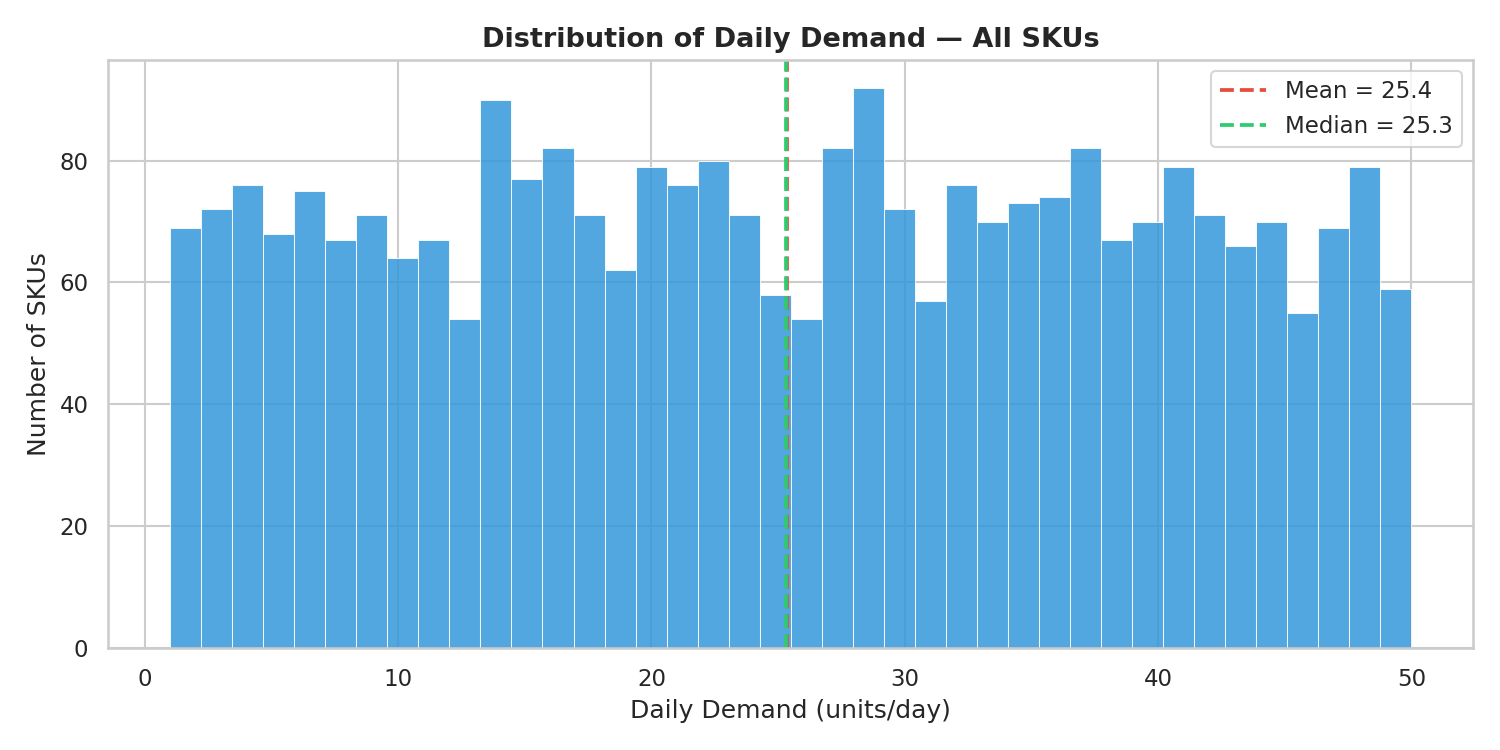
\includegraphics[width=\textwidth]{eda/01_demand_distribution.png}
    \caption{Daily demand distribution (near-uniform).}
    \label{fig:eda-demand}
\end{subfigure}
\hfill
\begin{subfigure}[b]{0.48\textwidth}
    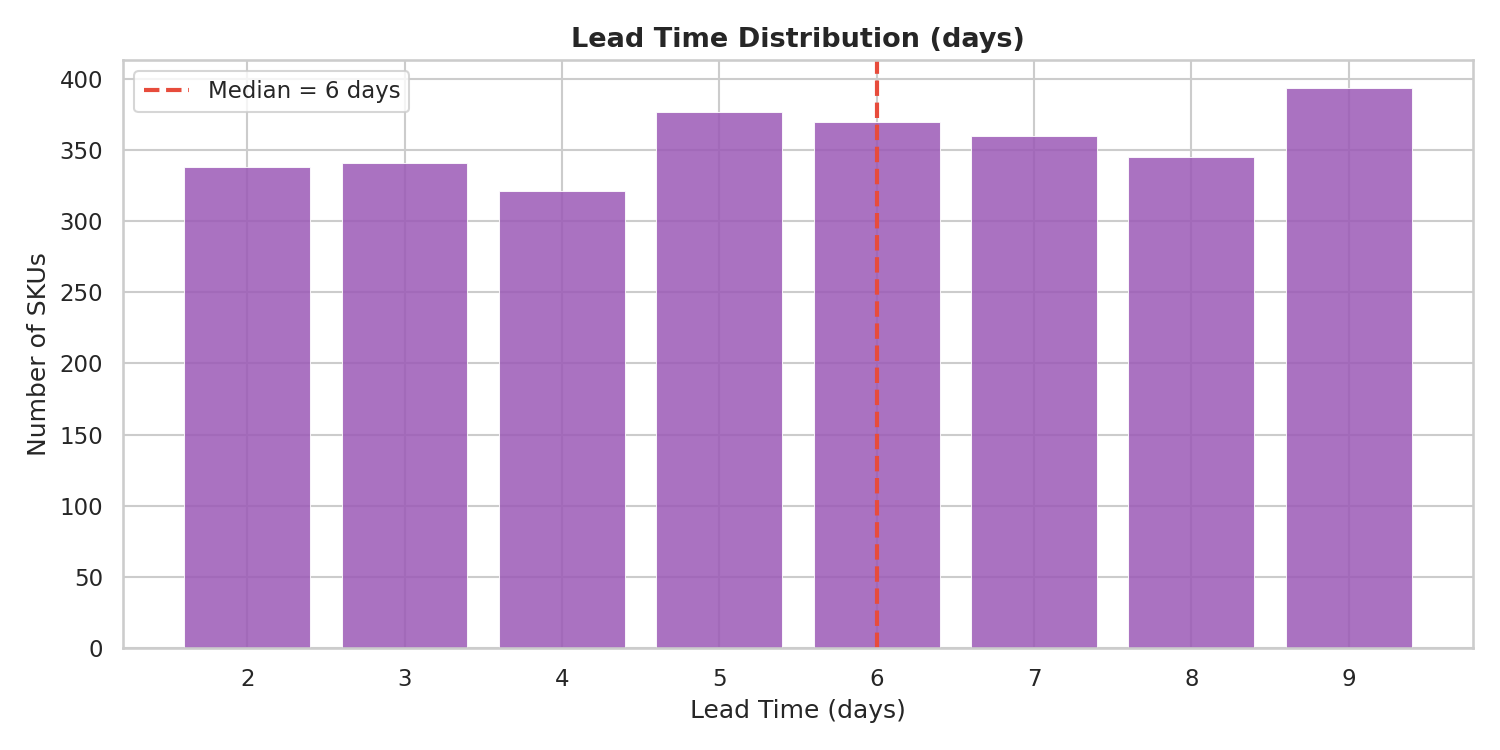
\includegraphics[width=\textwidth]{eda/04_lead_time_dist.png}
    \caption{Lead time distribution (uniform 2--9 days).}
    \label{fig:eda-leadtime}
\end{subfigure}
\caption{Exploratory data analysis plots.}
\label{fig:eda}
\end{figure}

% ── Error Analysis Plots ──────────────────────────────────────────────
\begin{figure}[H]
\centering
\begin{subfigure}[b]{0.48\textwidth}
    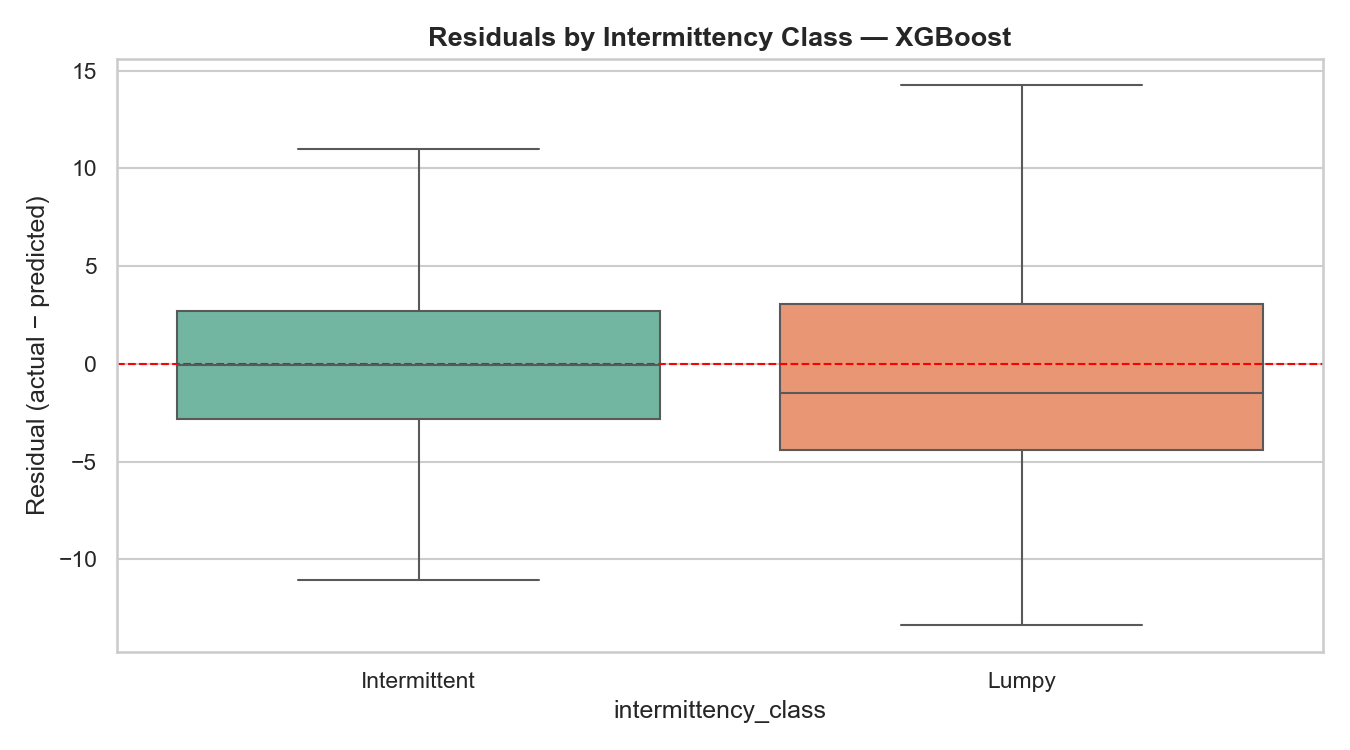
\includegraphics[width=\textwidth]{error_analysis/residuals_by_intermittency.png}
    \caption{Residuals by intermittency class.}
    \label{fig:error-analysis}
\end{subfigure}
\hfill
\begin{subfigure}[b]{0.48\textwidth}
    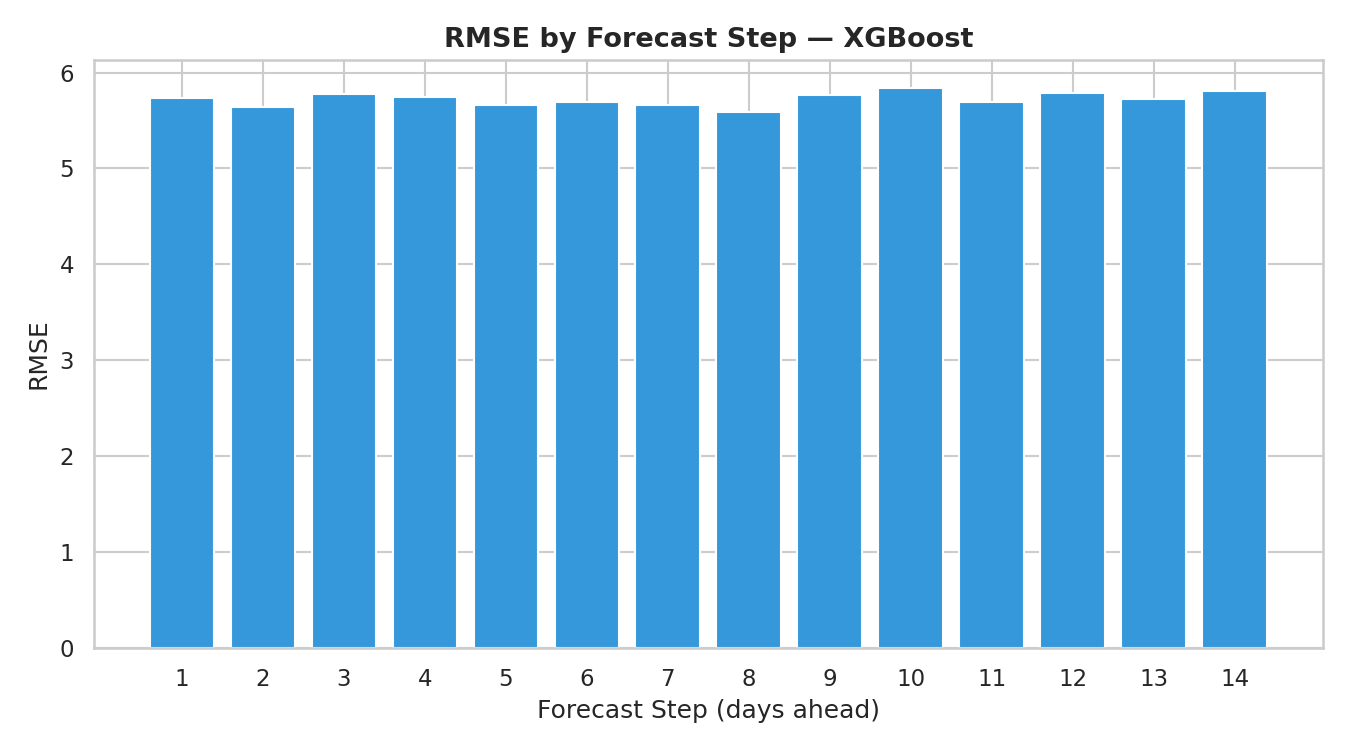
\includegraphics[width=\textwidth]{error_analysis/rmse_by_step.png}
    \caption{RMSE by forecast step (1--14).}
    \label{fig:rmse-step}
\end{subfigure}
\caption{Error analysis of the XGBoost forecast on the held-out test set.}
\end{figure}

% ── Prediction Intervals ─────────────────────────────────────────────
\begin{figure}[H]
\centering
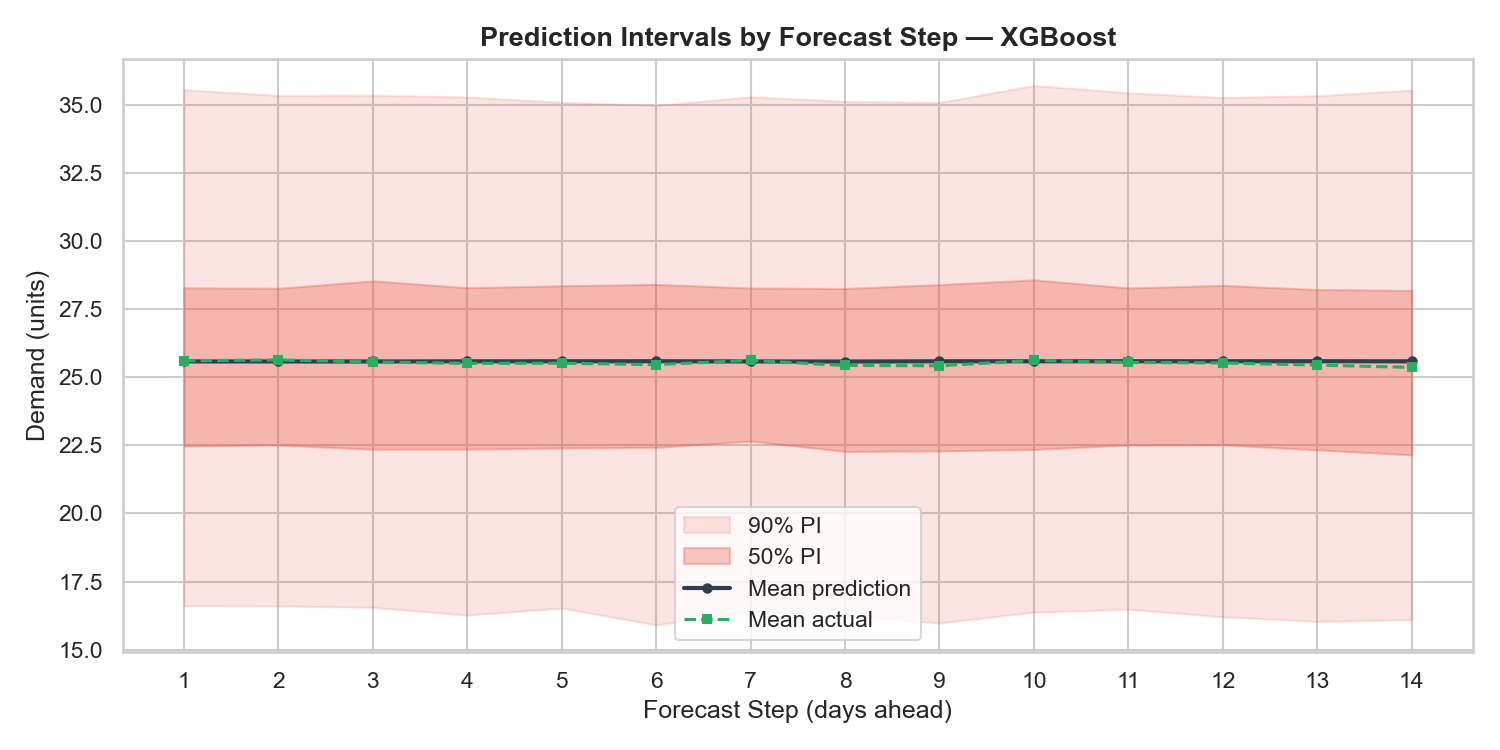
\includegraphics[width=0.78\textwidth]{error_analysis/prediction_intervals.png}
\caption{Prediction intervals by forecast step. 50\% PI (dark) and 90\% PI (light) around mean prediction. Green dashed: mean actual.}
\label{fig:pi}
\end{figure}

% ── Feature Importance ────────────────────────────────────────────────
\begin{figure}[H]
\centering
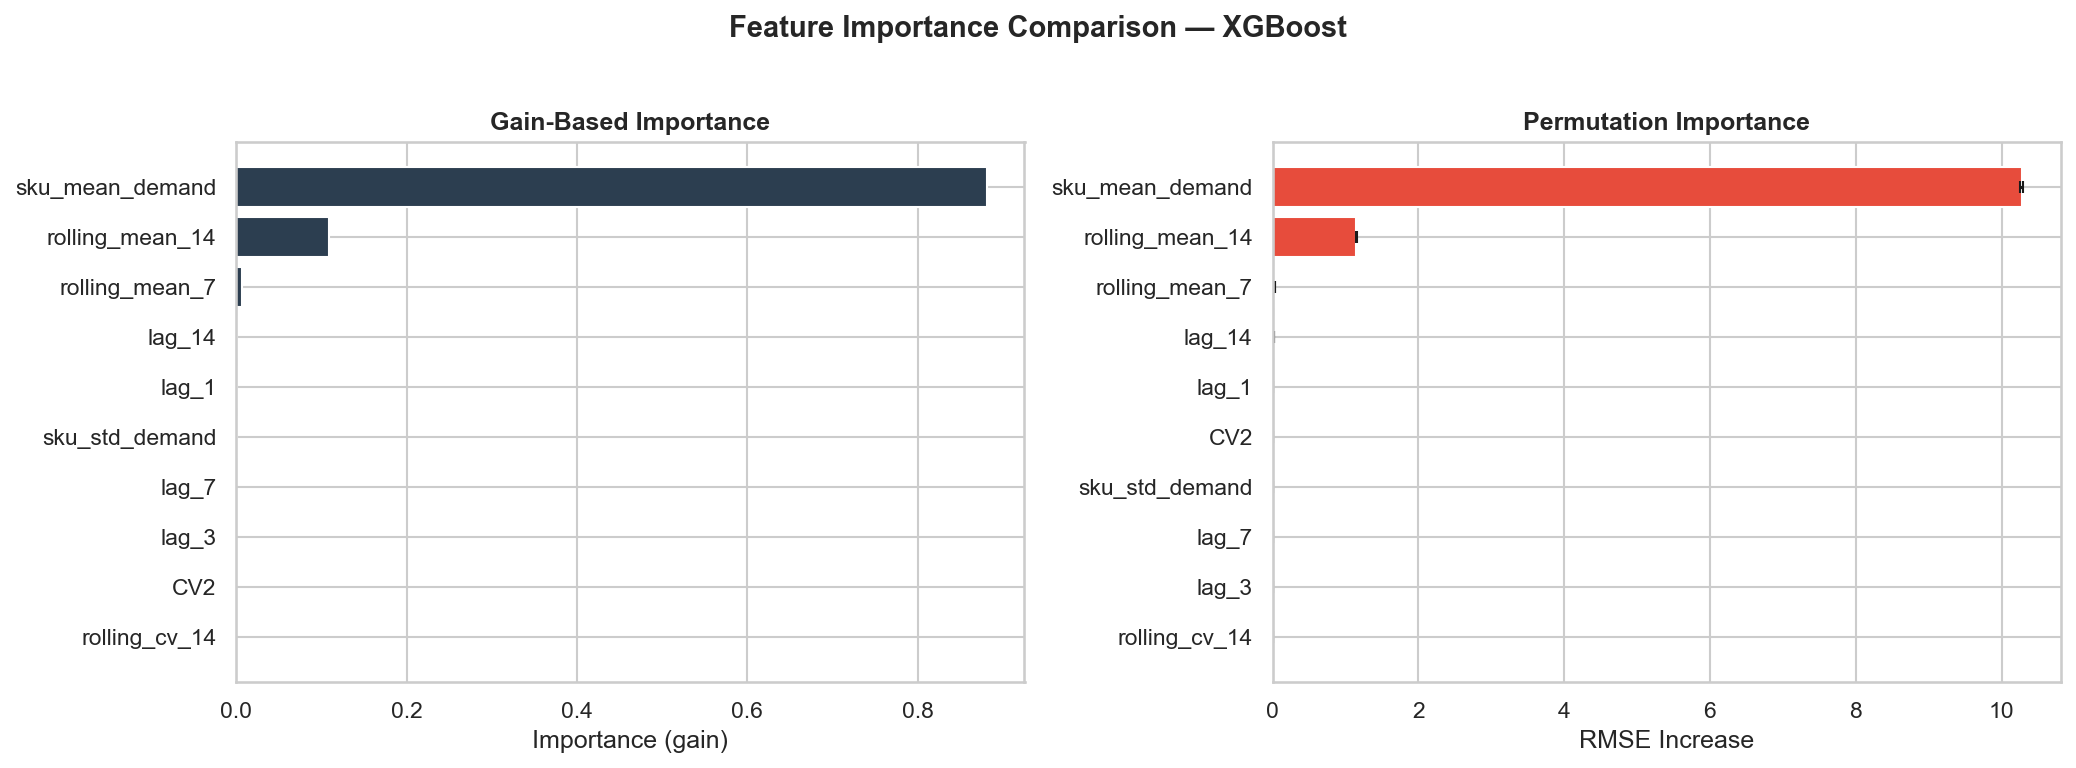
\includegraphics[width=0.88\textwidth]{error_analysis/importance_comparison.png}
\caption{Feature importance: gain-based (left) vs.\ permutation (right). Error bars: $\pm 1$ std across 5 repeats.}
\label{fig:importance-comparison}
\end{figure}

% ── Sensitivity Analysis ─────────────────────────────────────────────
\begin{figure}[H]
\centering
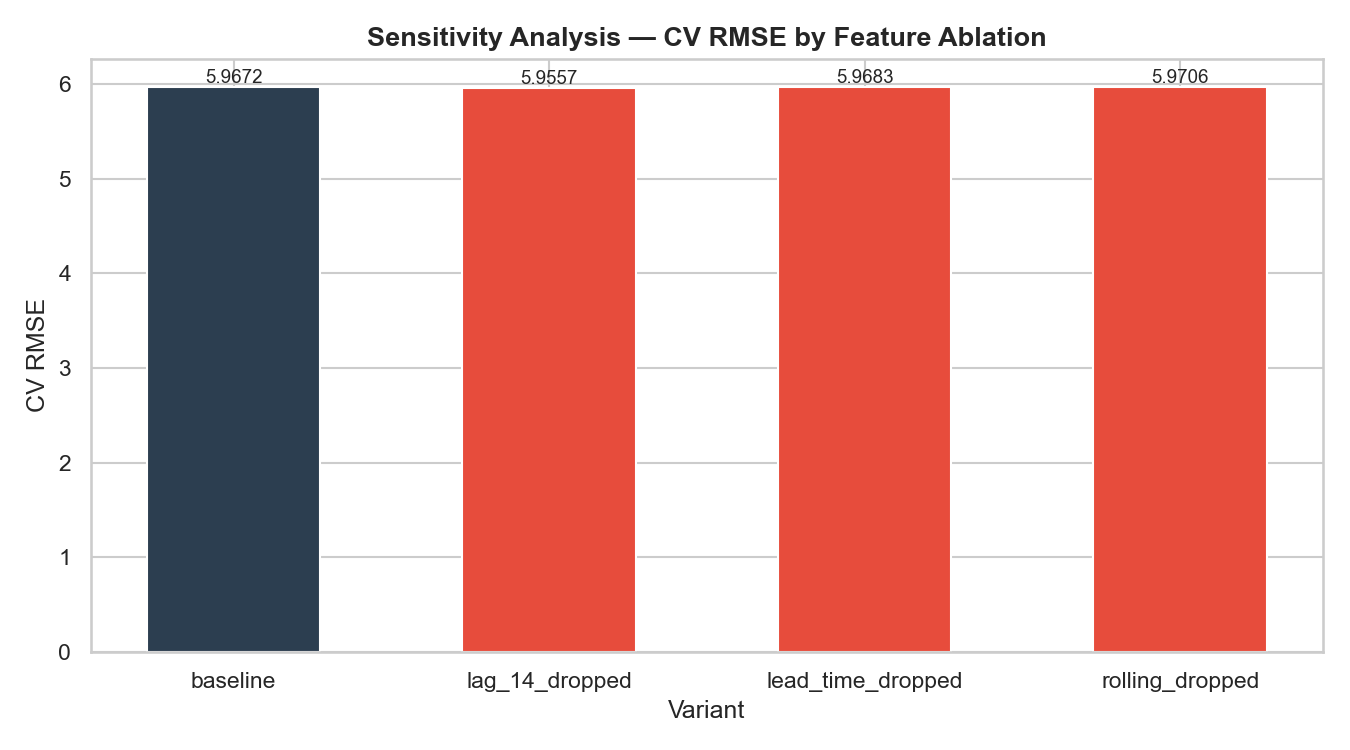
\includegraphics[width=0.65\textwidth]{error_analysis/sensitivity_analysis.png}
\caption{CV RMSE by feature ablation variant.}
\label{fig:sensitivity}
\end{figure}

% ── Supporting Tables ─────────────────────────────────────────────────

\begin{table}[H]
\centering
\caption{Model feature set (21 features).}
\label{tab:features}
\small
\begin{tabular}{@{}clll@{}}
\toprule
\textbf{\#} & \textbf{Feature} & \textbf{Type} & \textbf{Rationale} \\
\midrule
1  & \texttt{lag\_1}            & Lag       & Prior day demand \\
2  & \texttt{lag\_3}            & Lag       & 3-day trend \\
3  & \texttt{lag\_7}            & Lag       & Weekly periodicity \\
4  & \texttt{lag\_14}           & Lag       & Biweekly cycle \\
5  & \texttt{rolling\_mean\_7}  & Rolling   & 7-day average \\
6  & \texttt{rolling\_std\_7}   & Rolling   & 7-day variability \\
7  & \texttt{rolling\_mean\_14} & Rolling   & 14-day average \\
8  & \texttt{rolling\_std\_14}  & Rolling   & 14-day variability \\
9  & \texttt{rolling\_cv\_14}   & Rolling   & Coefficient of variation \\
10 & \texttt{day\_of\_week}     & Calendar  & Mon=0 \ldots\ Sun=6 \\
11 & \texttt{week\_of\_year}    & Calendar  & ISO week (1--53) \\
12 & \texttt{month}             & Calendar  & Month (1--12) \\
13 & \texttt{is\_weekend}       & Calendar  & Binary flag \\
14 & \texttt{sku\_mean\_demand} & Static    & Historical mean \\
15 & \texttt{sku\_std\_demand}  & Static    & Historical std \\
16 & \texttt{sku\_mean\_lead\_time} & Static & Mean lead time \\
17 & \texttt{sku\_reorder\_freq} & Static   & Reorder frequency \\
18 & \texttt{ADI}               & Interm.   & Avg Demand Interval \\
19 & \texttt{CV\textsuperscript{2}} & Interm. & Sq.\ coeff.\ of variation \\
20 & \texttt{category\_enc}     & Cat.      & Encoded category \\
21 & \texttt{intermittency\_enc} & Cat.     & Encoded class \\
\bottomrule
\end{tabular}
\end{table}

\begin{table}[H]
\centering
\caption{Top 10 features by permutation importance (RMSE increase when shuffled, 5 repeats).}
\label{tab:perm-importance}
\small
\begin{tabular}{@{}clcc@{}}
\toprule
\textbf{Rank} & \textbf{Feature} & \textbf{RMSE $\Delta$} & \textbf{Std} \\
\midrule
1  & \texttt{sku\_mean\_demand}  & +10.275 & $\pm$0.026 \\
2  & \texttt{rolling\_mean\_14}  & +1.150  & $\pm$0.005 \\
3  & \texttt{rolling\_mean\_7}   & +0.033  & $\pm$0.002 \\
4  & \texttt{lag\_14}            & +0.020  & $\pm$0.001 \\
5  & \texttt{lag\_1}             & +0.007  & $\pm$0.000 \\
6  & \texttt{CV\textsuperscript{2}} & +0.006 & $\pm$0.001 \\
7  & \texttt{sku\_std\_demand}   & +0.004  & $\pm$0.000 \\
8  & \texttt{lag\_7}             & +0.003  & $\pm$0.000 \\
9  & \texttt{lag\_3}             & +0.003  & $\pm$0.001 \\
10 & \texttt{rolling\_cv\_14}    & +0.002  & $\pm$0.000 \\
\bottomrule
\end{tabular}
\end{table}

\begin{table}[H]
\centering
\caption{Top 5 SKUs by cost saving.}
\label{tab:top5}
\small
\begin{tabular}{@{}cllrrrl@{}}
\toprule
 & \textbf{SKU} & \textbf{Category} & \textbf{Dynamic} & \textbf{Static} & \textbf{Saving} & \textbf{Action} \\
\midrule
1 & ITM10409 & Pharma    & \$127,160 & \$278,938 & 54.4\% & Hold \\
2 & ITM12384 & Groceries & \$120,370 & \$263,443 & 54.3\% & Hold \\
3 & ITM11647 & Pharma    & \$112,651 & \$246,370 & 54.3\% & Hold \\
4 & ITM11613 & Pharma    & \$105,355 & \$230,369 & 54.3\% & Reorder \\
5 & ITM12063 & Apparel   & \$114,863 & \$250,841 & 54.2\% & Reorder \\
\bottomrule
\end{tabular}
\end{table}

\begin{table}[H]
\centering
\caption{Forecast error to cost propagation. Multiplier 1.0$\times$ = current model.}
\label{tab:error-propagation}
\small
\begin{tabular}{@{}rrrrc@{}}
\toprule
\textbf{Mult.} & \textbf{Avg SS} & \textbf{Total Cost} & \textbf{Cost $\Delta$} & \textbf{Reorder} \\
\midrule
0.25$\times$ & 63.1 & \$130,865,288 & $-0.01\%$ & 1,090 \\
0.50$\times$ & 63.1 & \$130,867,364 & $-0.01\%$ & 1,090 \\
1.00$\times$ & 63.1 & \$130,875,651 & 0.00\%    & 1,090 \\
1.50$\times$ & 63.1 & \$130,889,409 & $+0.01\%$ & 1,090 \\
2.00$\times$ & 63.1 & \$130,908,561 & $+0.03\%$ & 1,090 \\
3.00$\times$ & 63.2 & \$130,962,625 & $+0.07\%$ & 1,090 \\
\bottomrule
\end{tabular}
\end{table}

% ══════════════════════════════════════════════════════════════════════
%  APPENDIX B — Dashboard Screenshots
% ══════════════════════════════════════════════════════════════════════
\newpage
\section{Appendix: Dashboard Screenshots}
\label{sec:appendix-dashboard}

The following screenshots document the interactive Streamlit dashboard
(\texttt{dashboard/app.py}) that serves as the decision-support interface for
the inventory optimisation system. The dashboard provides four main tabs plus
configurable sidebar controls; all parameter changes propagate in real time.

% ── Demand Forecast ──────────────────────────────────────────────────
\subsection*{Demand Forecast}

\begin{figure}[H]
\centering
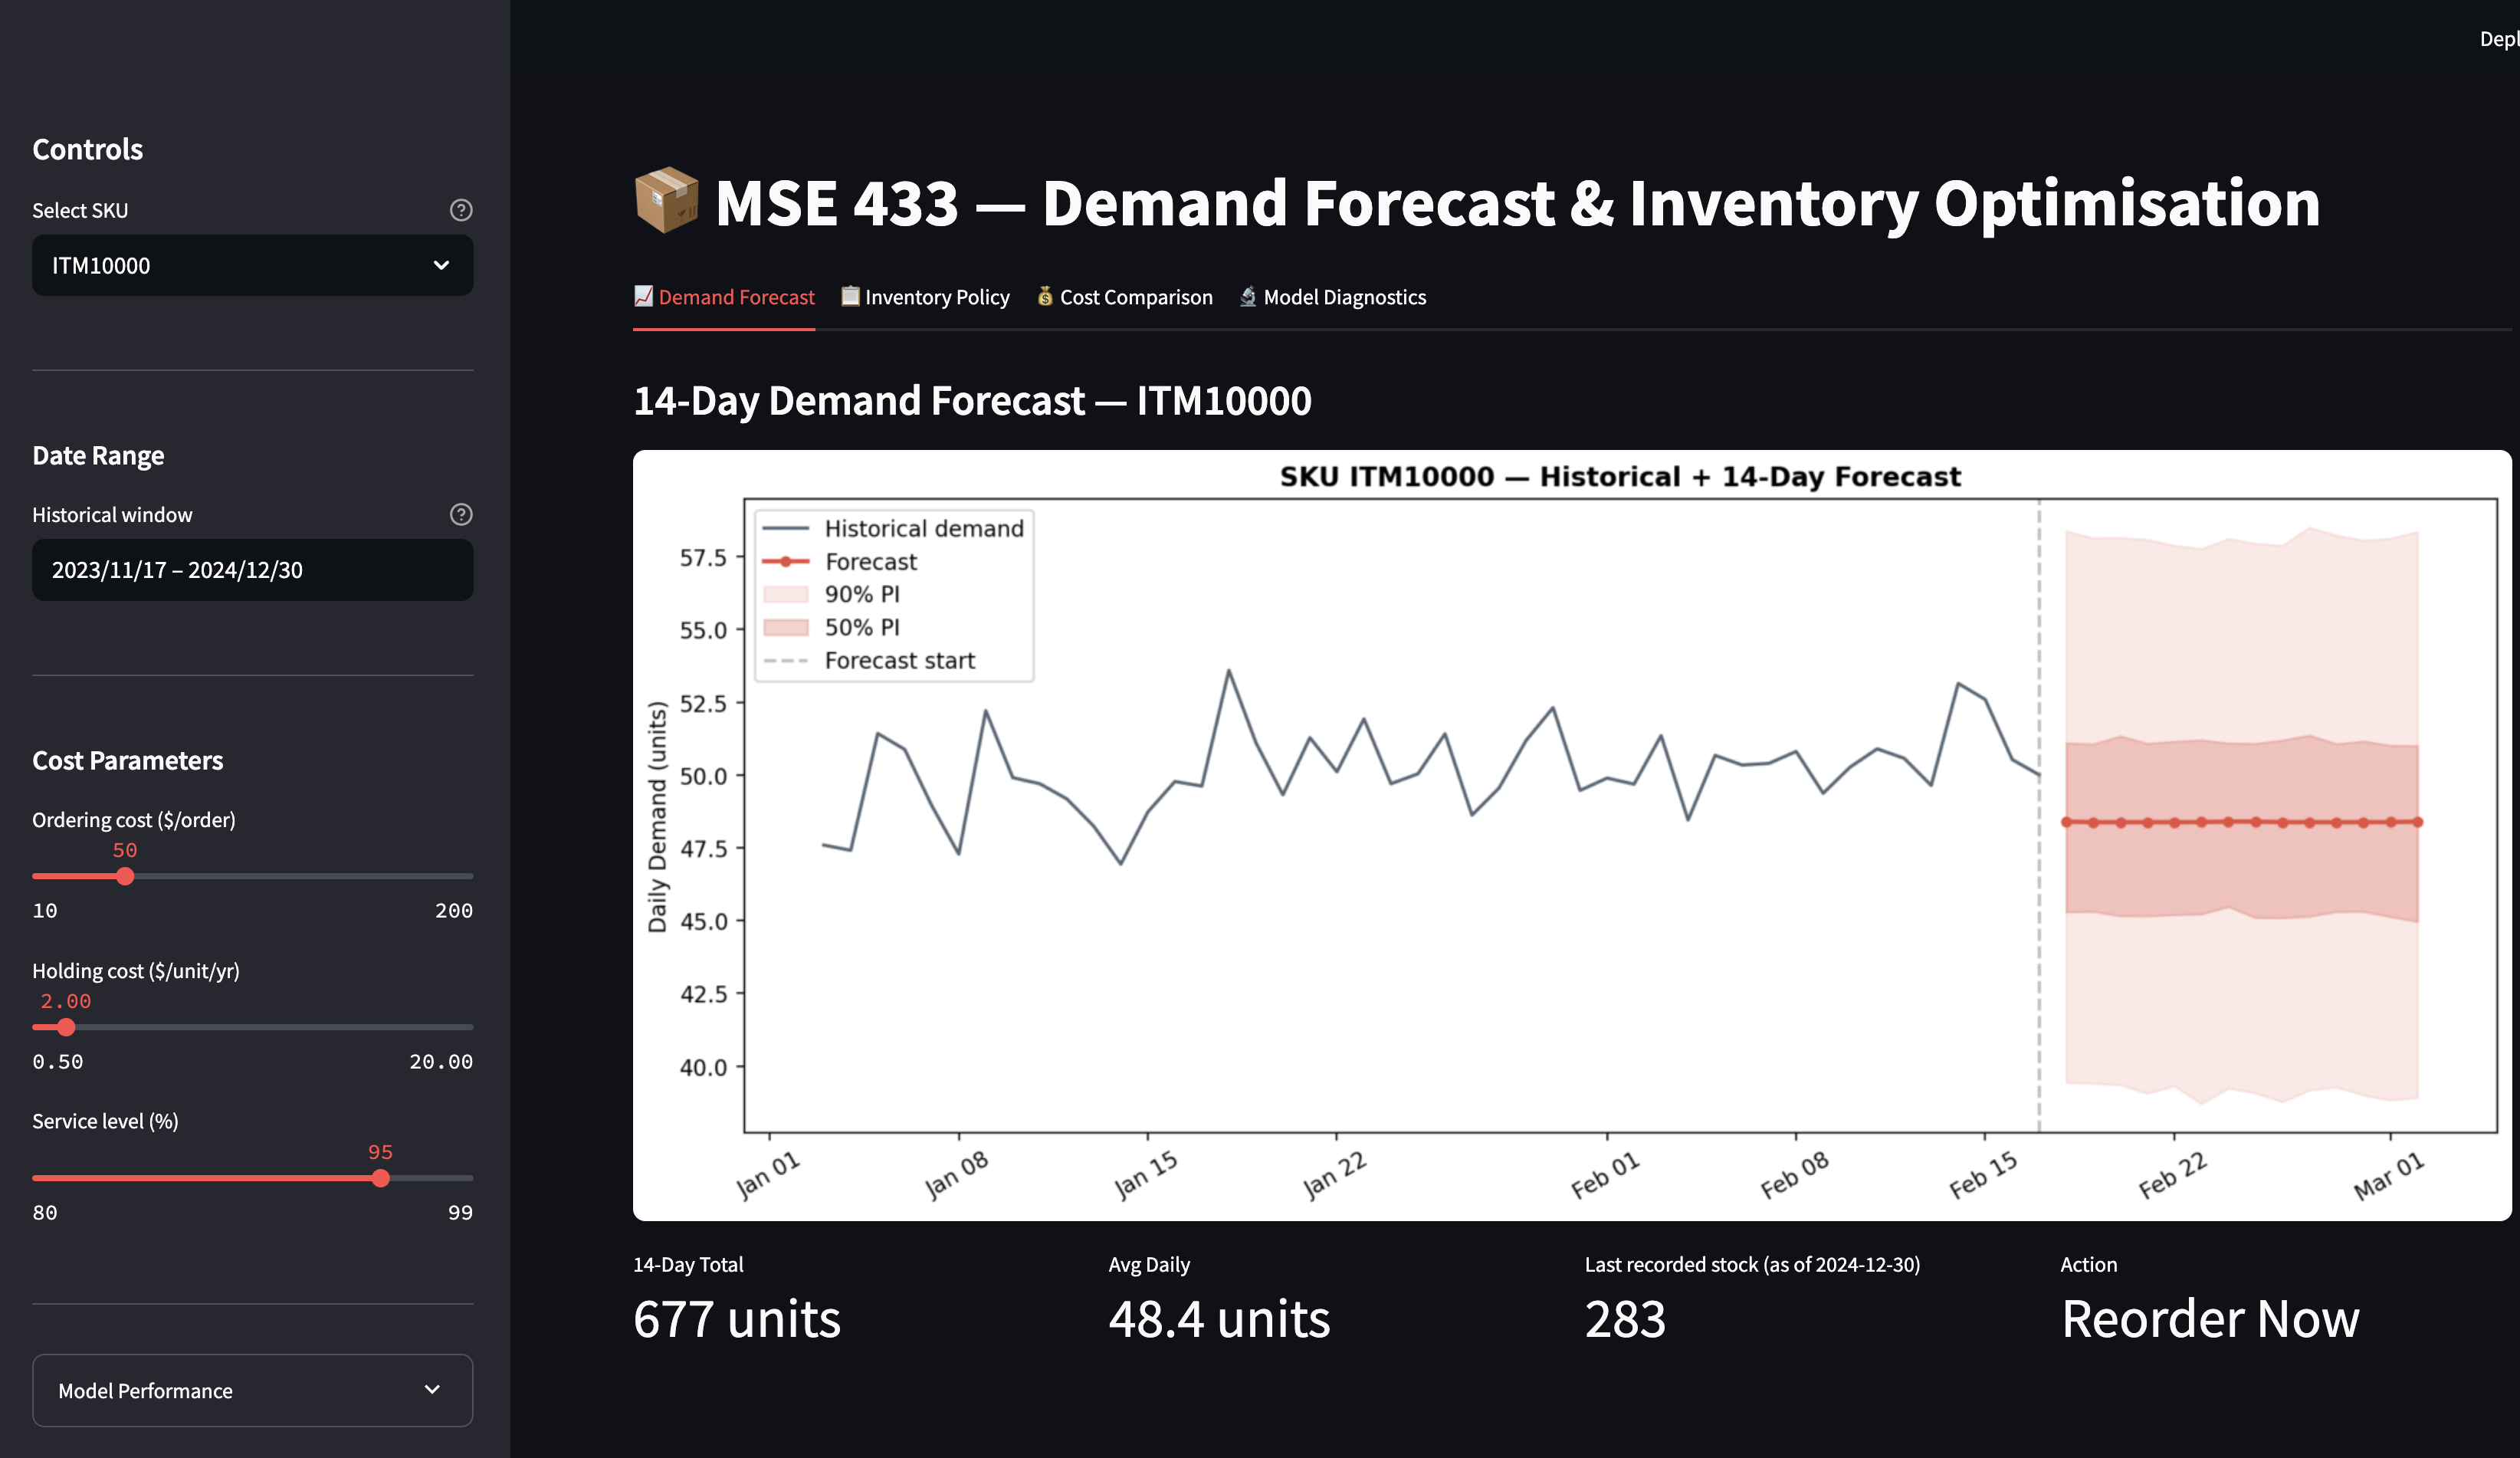
\includegraphics[width=\textwidth]{screenshots/forecast_tab.png}
\caption{Demand Forecast tab for SKU ITM10000. The left sidebar contains
controls; SKU selector, historical date range picker, cost parameter
sliders (ordering cost, holding cost, service level), and a collapsible
model performance summary. The main panel displays historical daily demand
(dark line), the 14-day recursive forecast (red line with markers), and
50\%/90\% prediction interval bands. Metric cards below summarise the
14-day total, average daily demand, last recorded stock level, and
recommended action.}
\label{fig:ss-forecast}
\end{figure}

% ── Inventory Policy ─────────────────────────────────────────────────
\subsection*{Inventory Policy}

\begin{figure}[H]
\centering
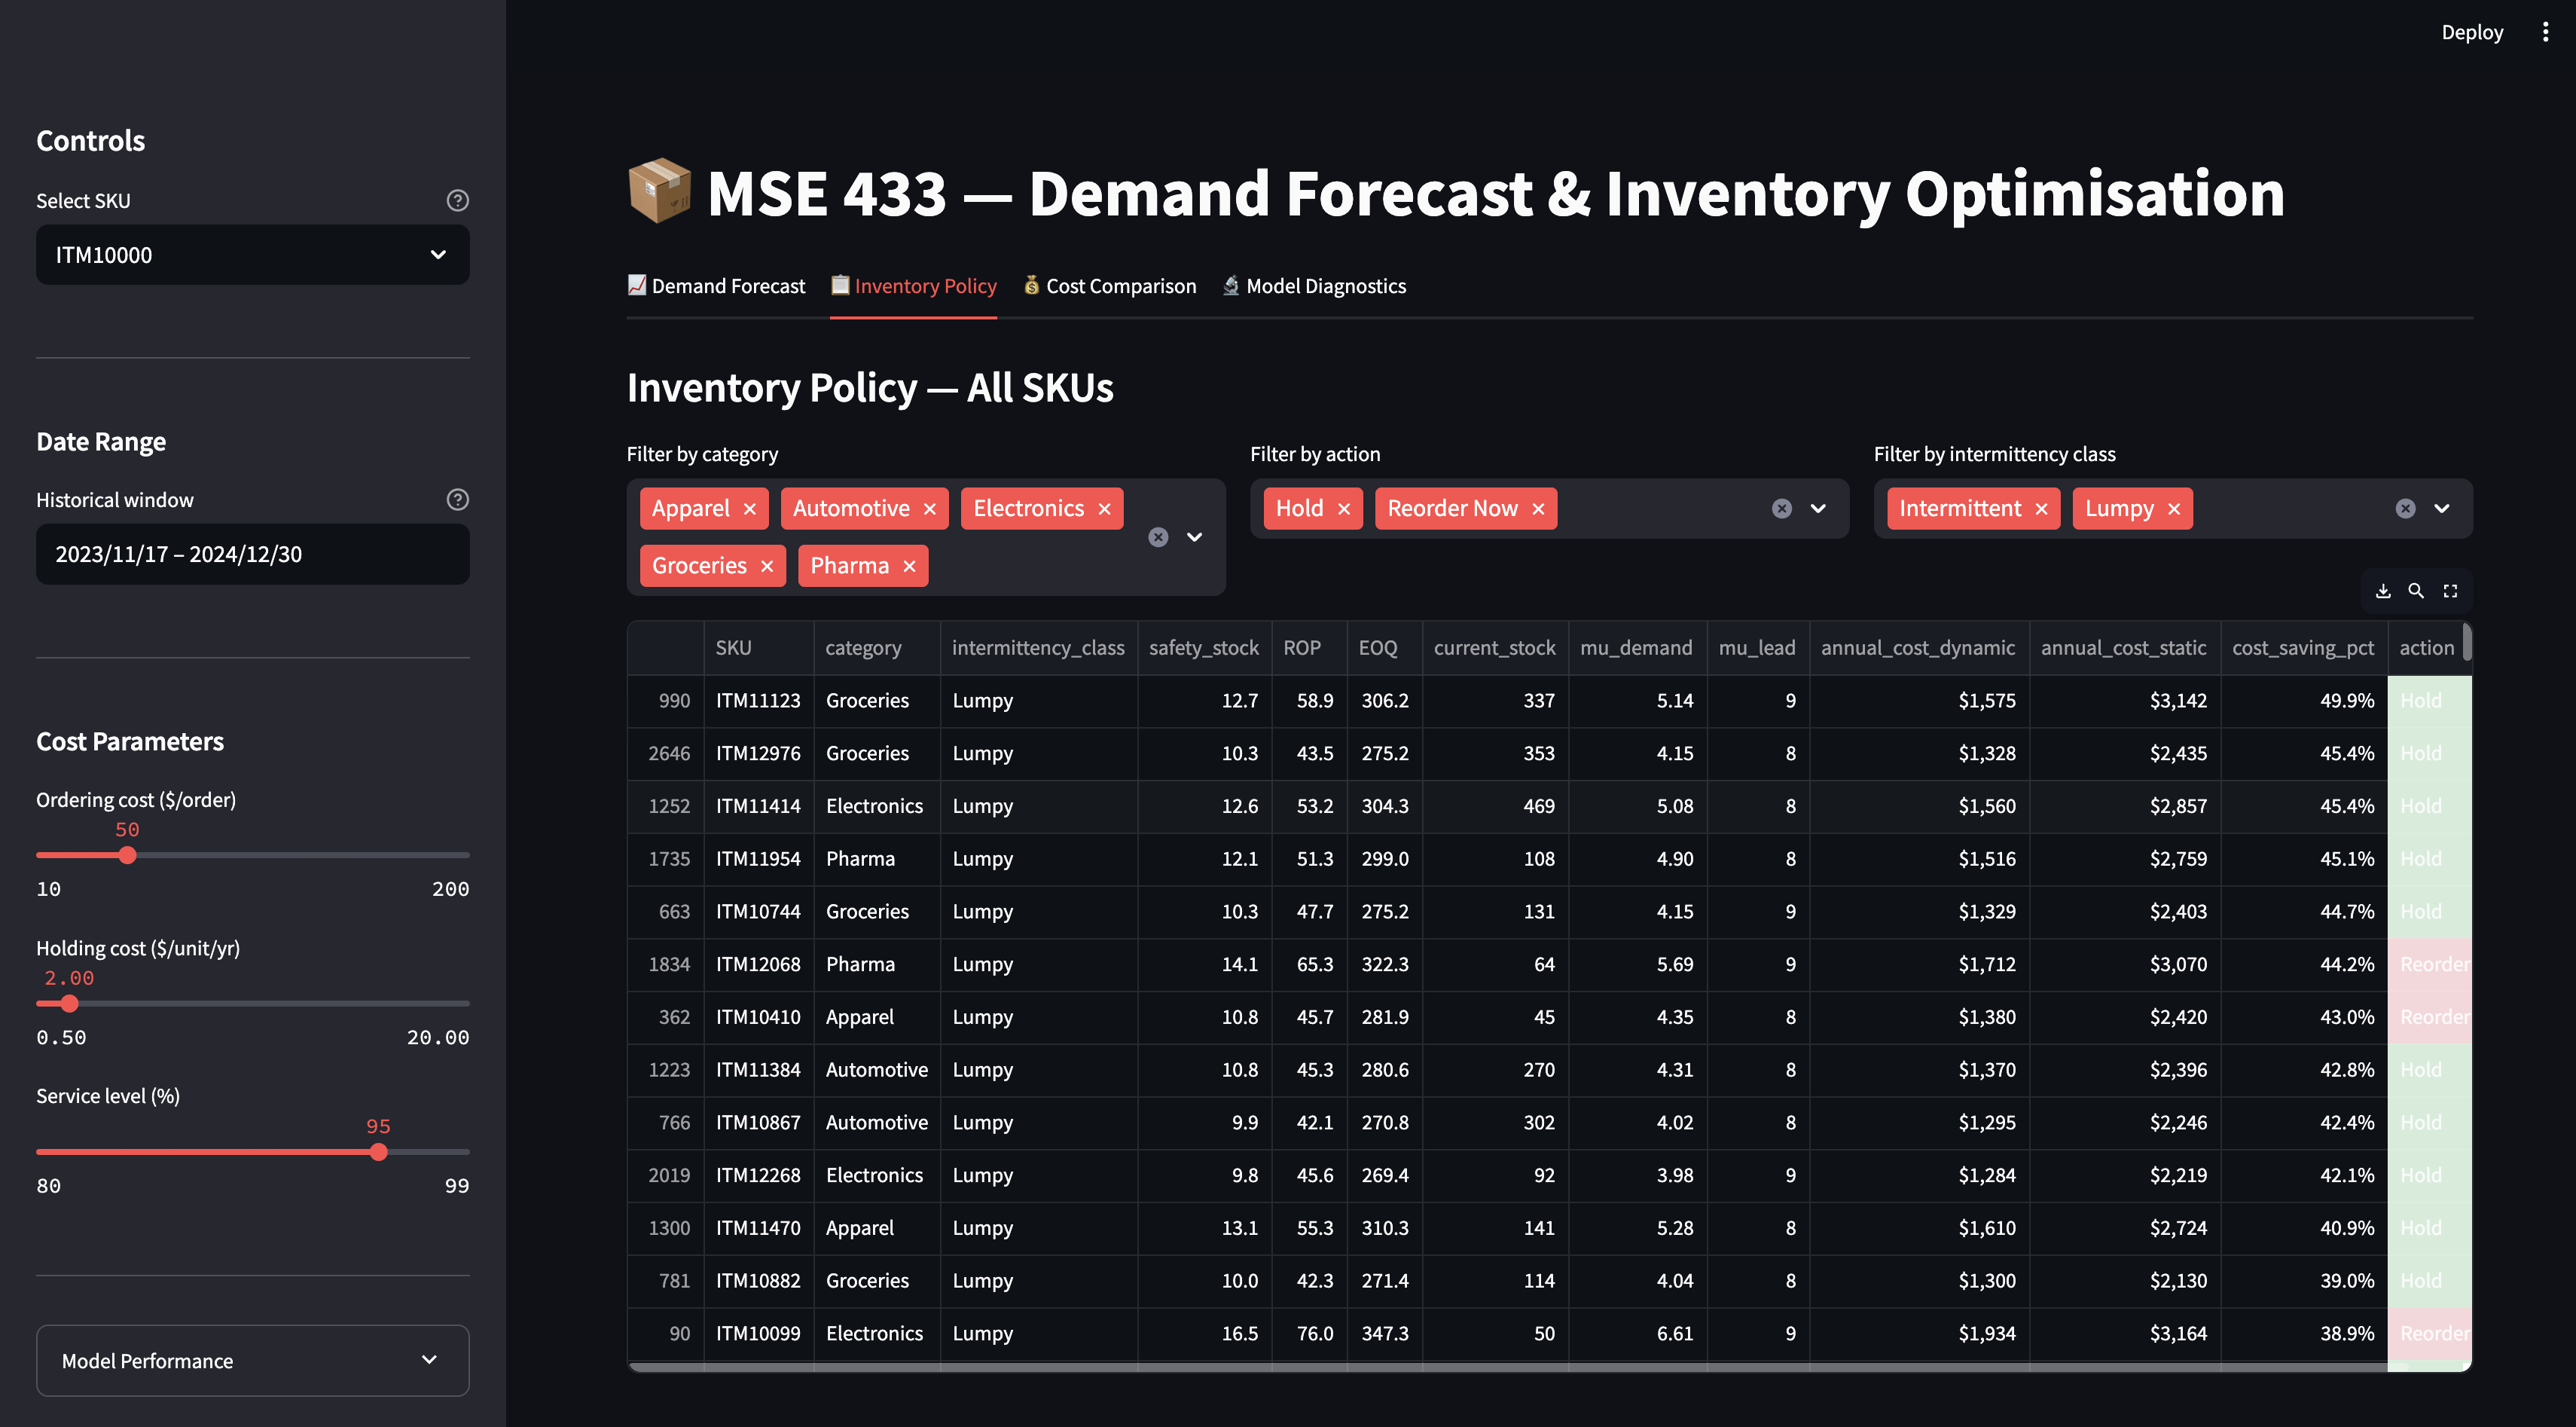
\includegraphics[width=\textwidth]{screenshots/policy_tab.png}
\caption{Inventory Policy tab. Rows are colour-coded: green = Hold,
red = Reorder Now. The table includes safety stock, reorder point (ROP),
economic order quantity (EOQ), current stock, and annual cost under the
dynamic policy. Multi-select filters for category, action, and
intermittency class appear above the table; aggregate metrics appear below.}
\label{fig:ss-policy}
\end{figure}

% ── Cost Comparison ──────────────────────────────────────────────────
\subsection*{Cost Comparison}

\begin{figure}[H]
\centering
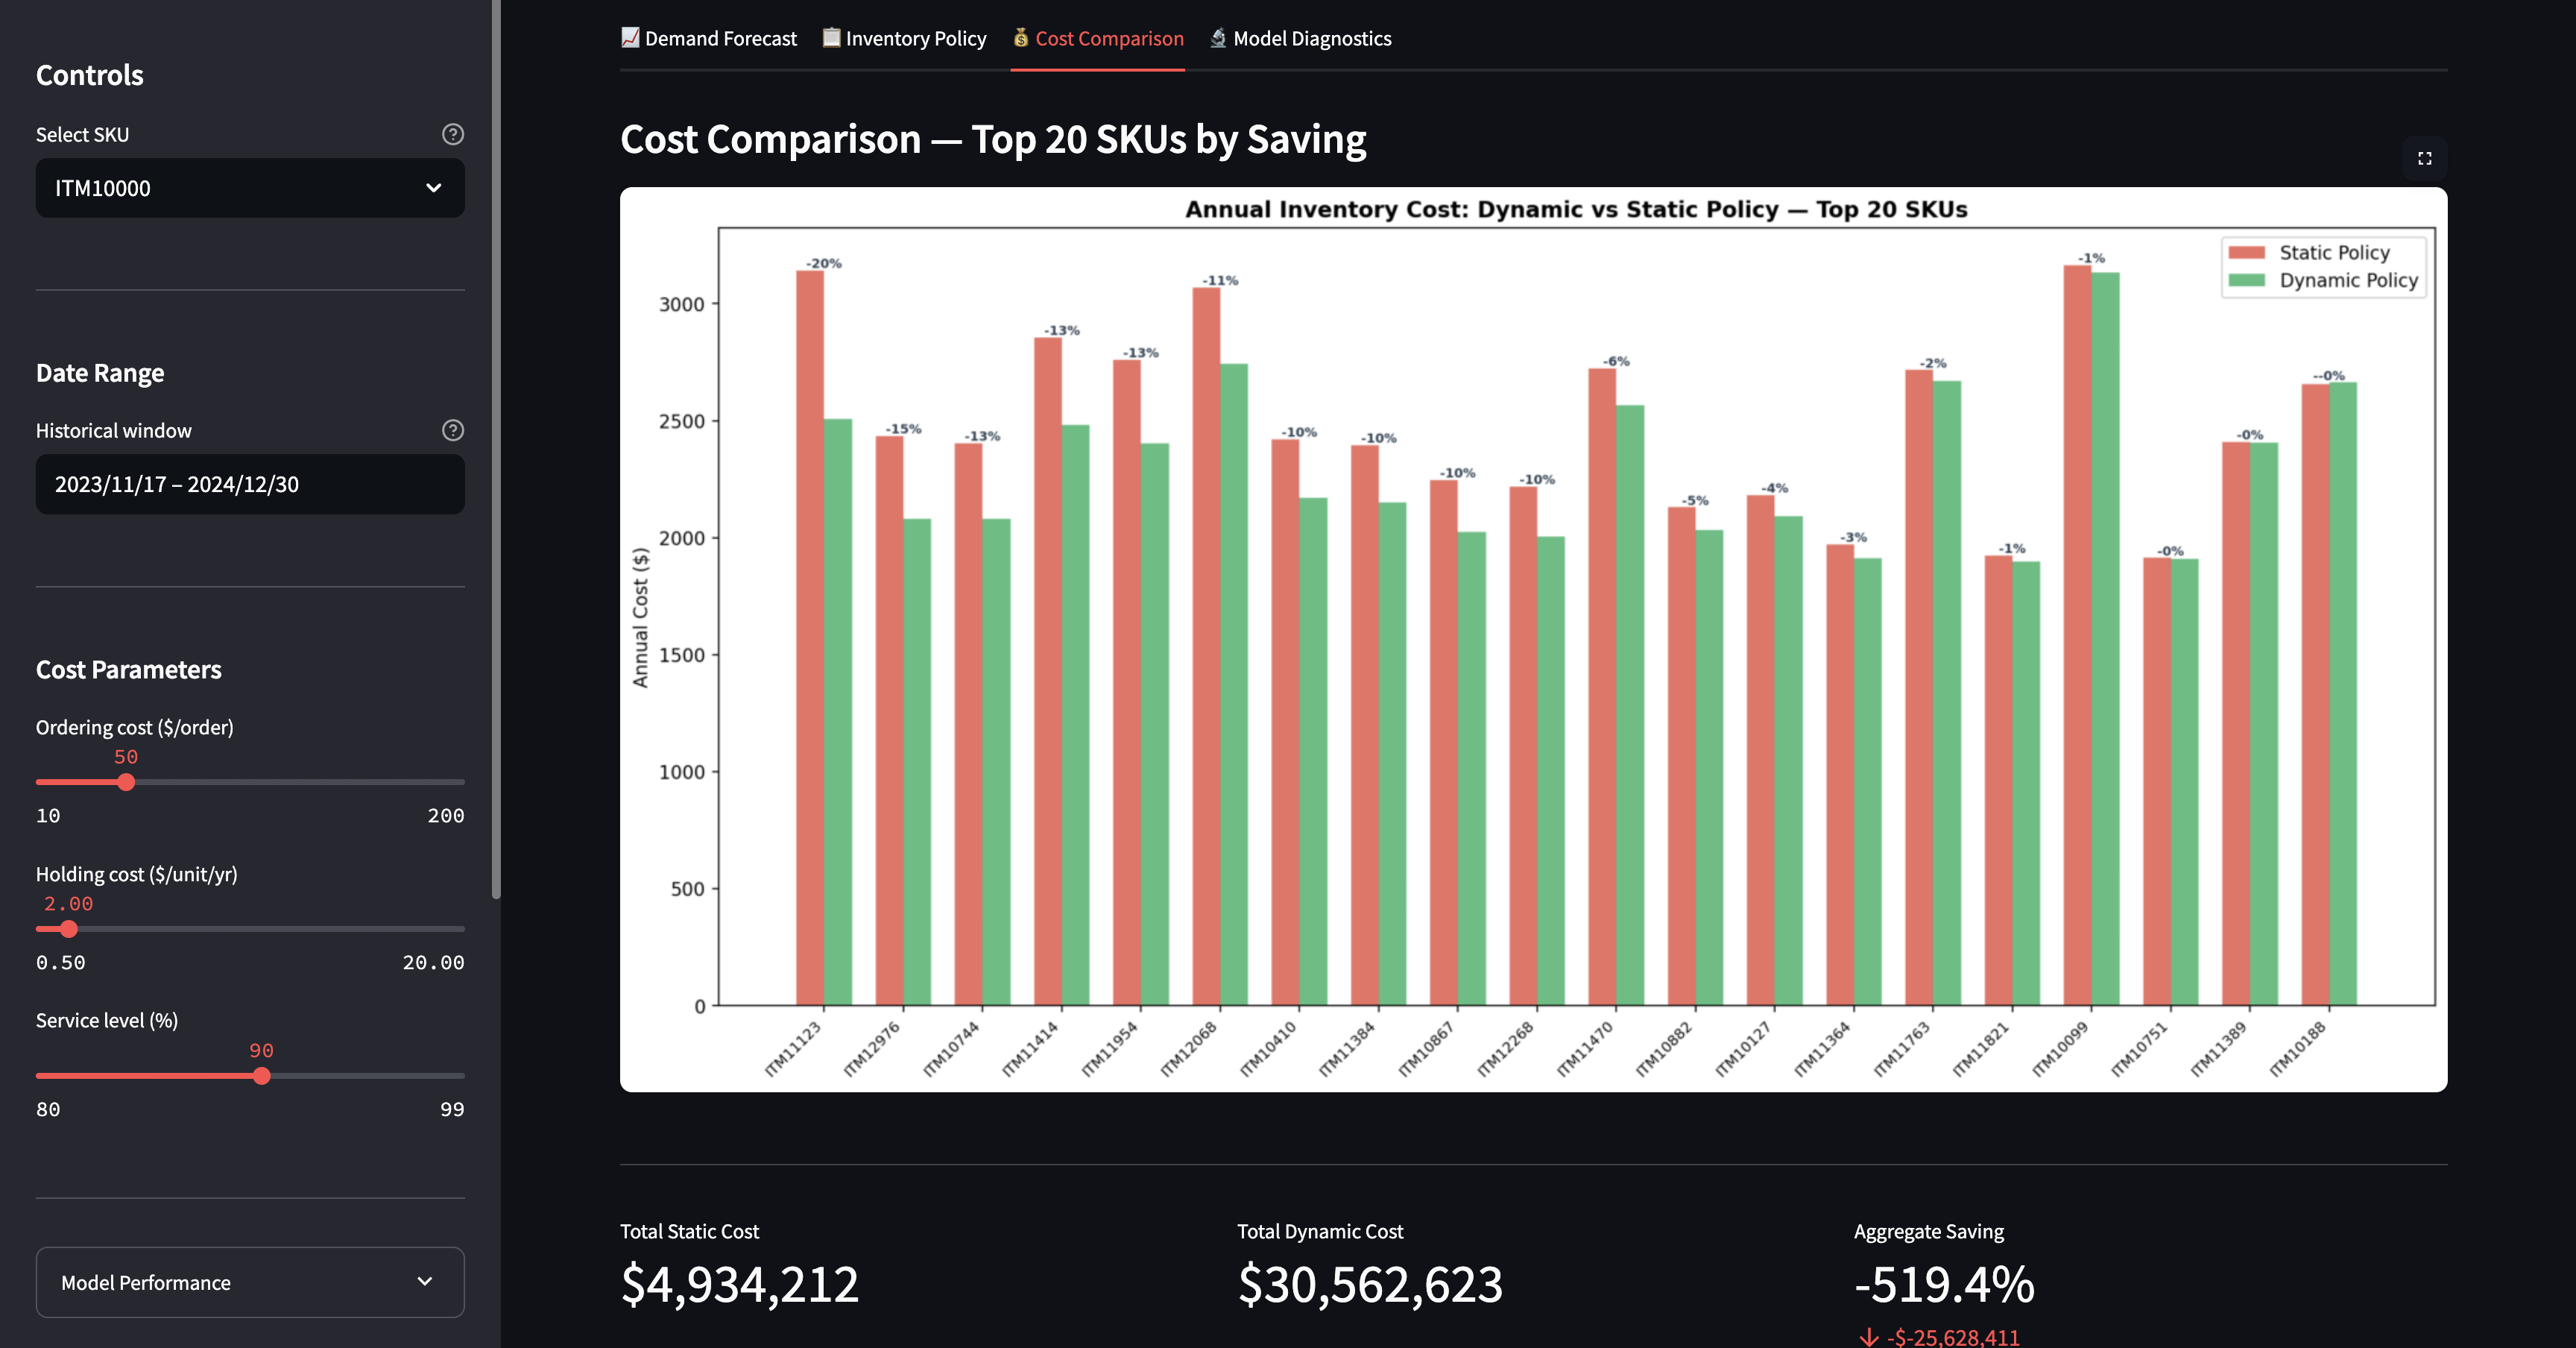
\includegraphics[width=\textwidth]{screenshots/cost_tab.png}
\caption{Cost Comparison tab. Grouped bar chart of the top 20 SKUs by
cost saving: static policy (red) vs.\ dynamic policy (green) with
percentage savings annotated above each pair. Summary cards show total
static cost, total dynamic cost, and aggregate saving.}
\label{fig:ss-cost}
\end{figure}

% ── Model Diagnostics ────────────────────────────────────────────────
\subsection*{Model Diagnostics}

\begin{figure}[H]
\centering
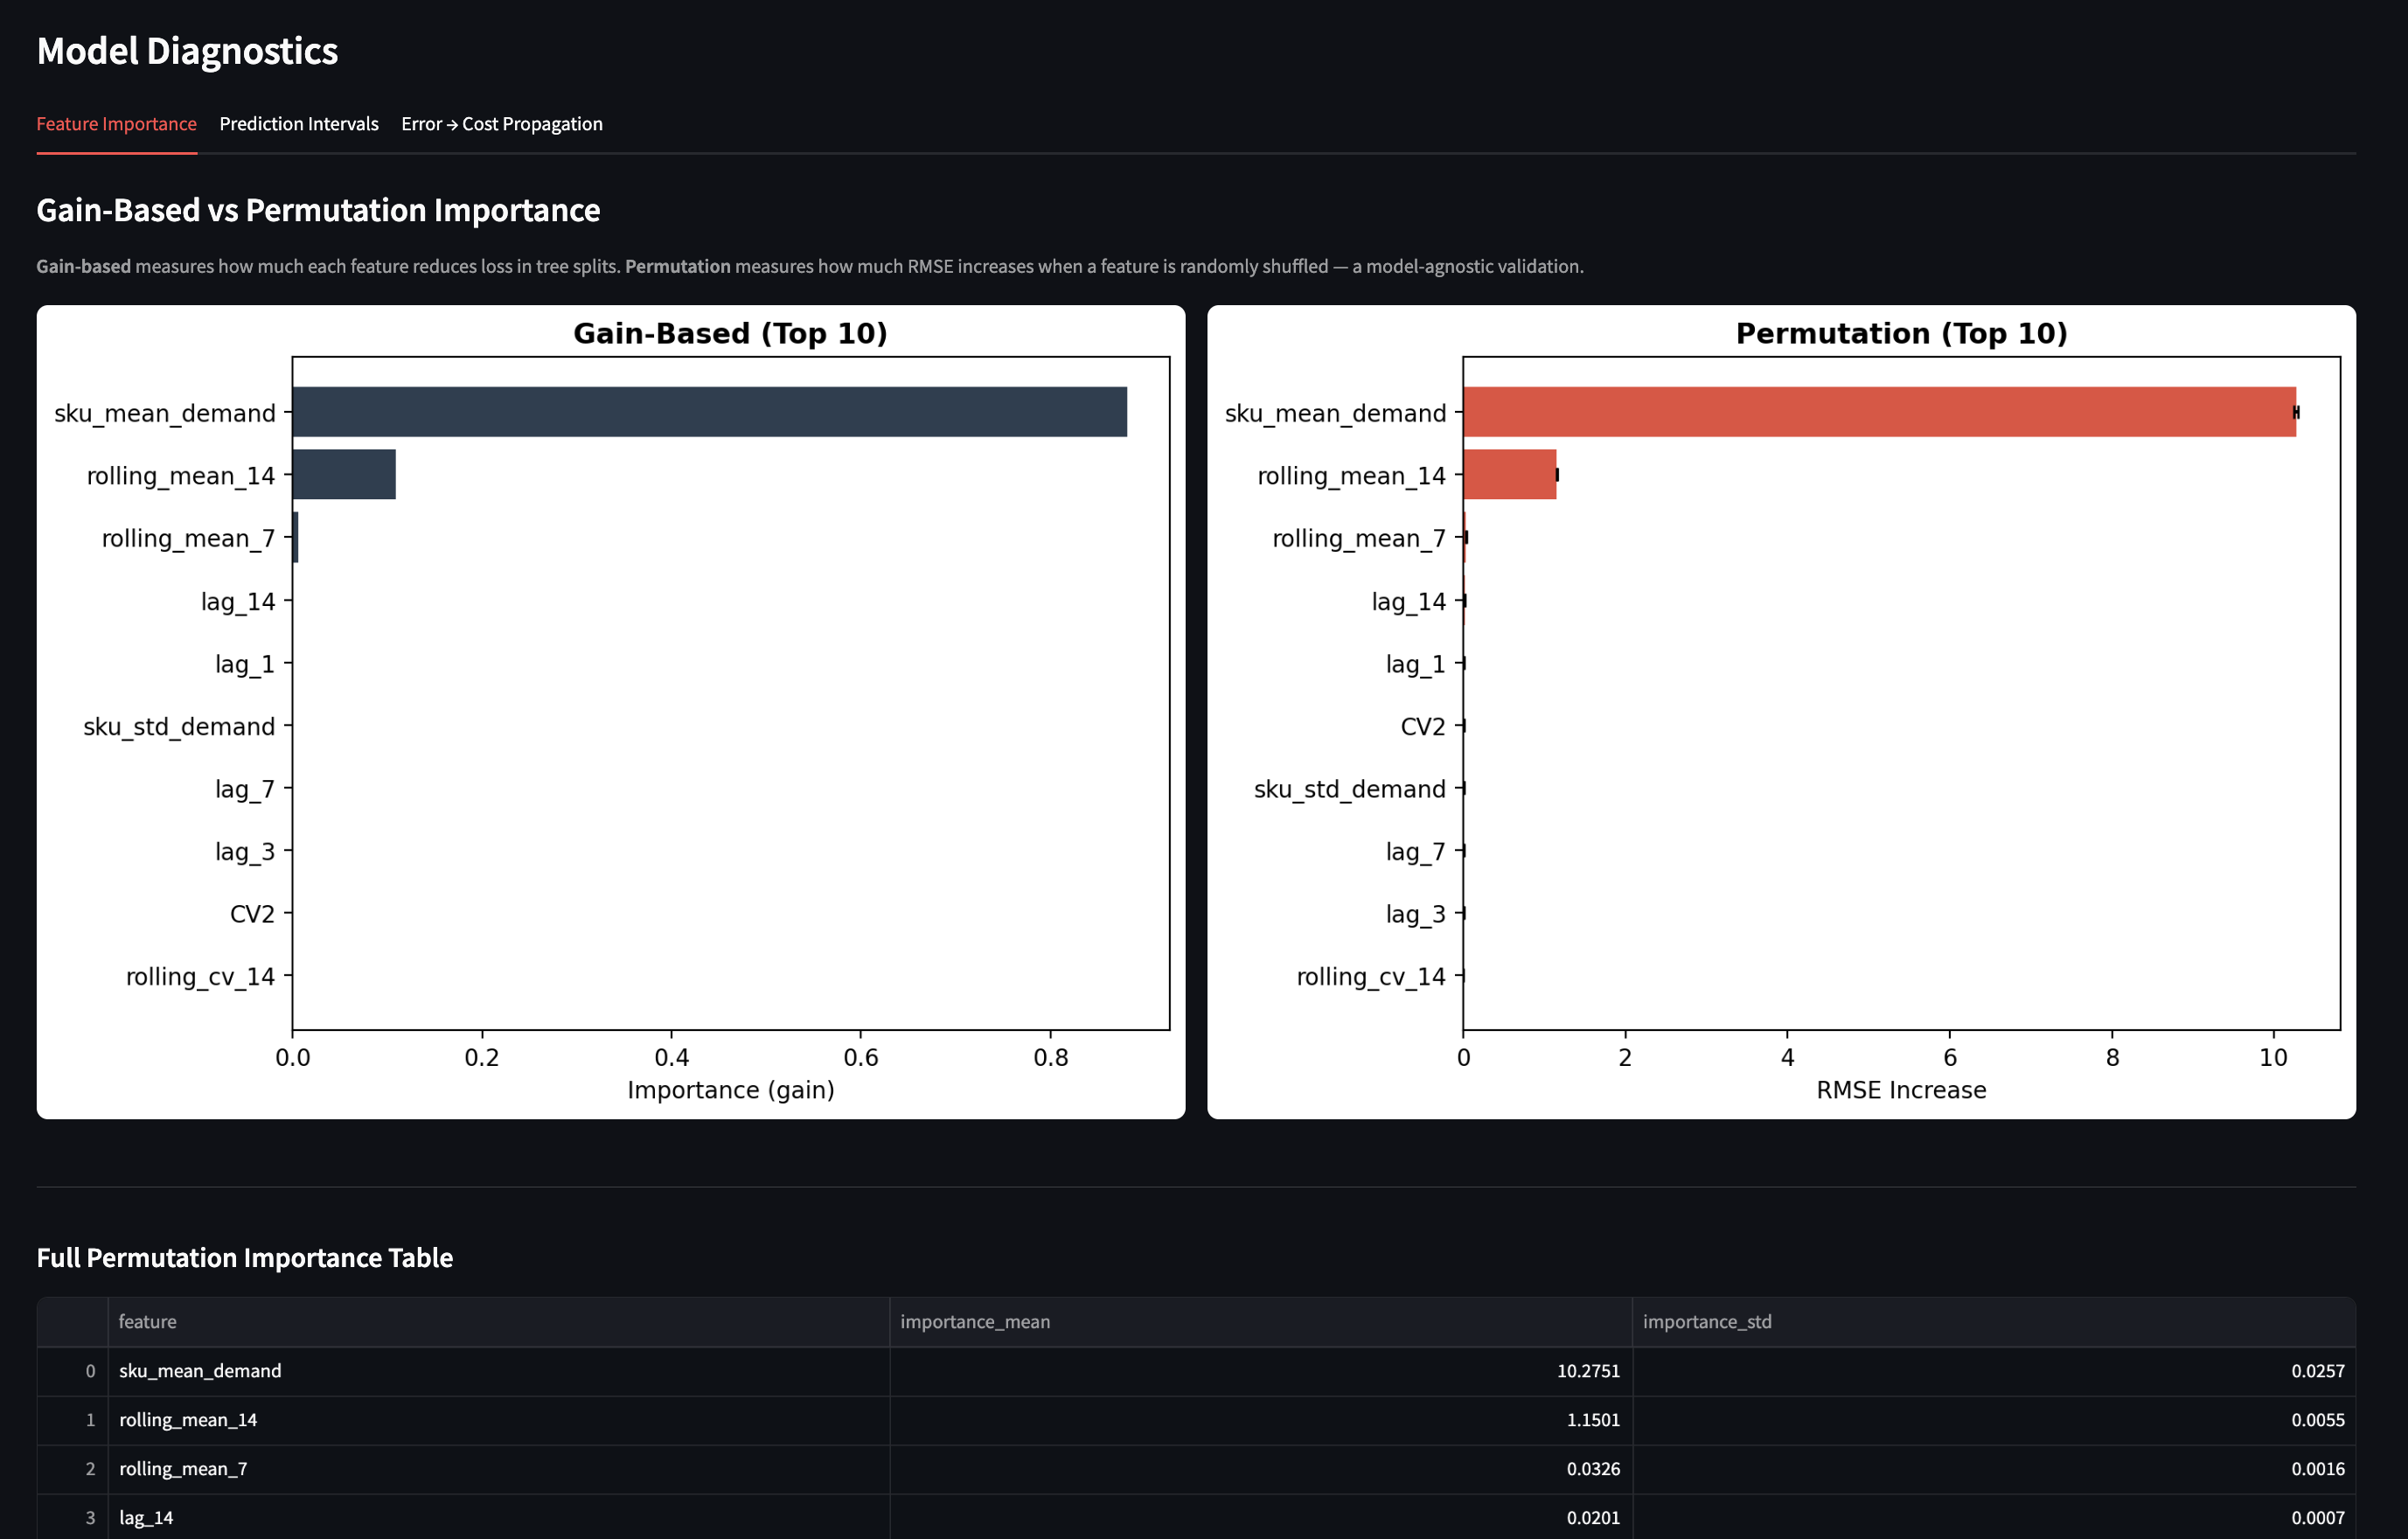
\includegraphics[width=\textwidth]{screenshots/diagnostics_feature_importance.png}
\caption{Feature Importance sub-tab. Side-by-side bar charts of gain-based
importance (left) and permutation importance with error bars (right) for
the top 10 features, with a full permutation importance table below.}
\label{fig:ss-importance}
\end{figure}

\begin{figure}[H]
\centering
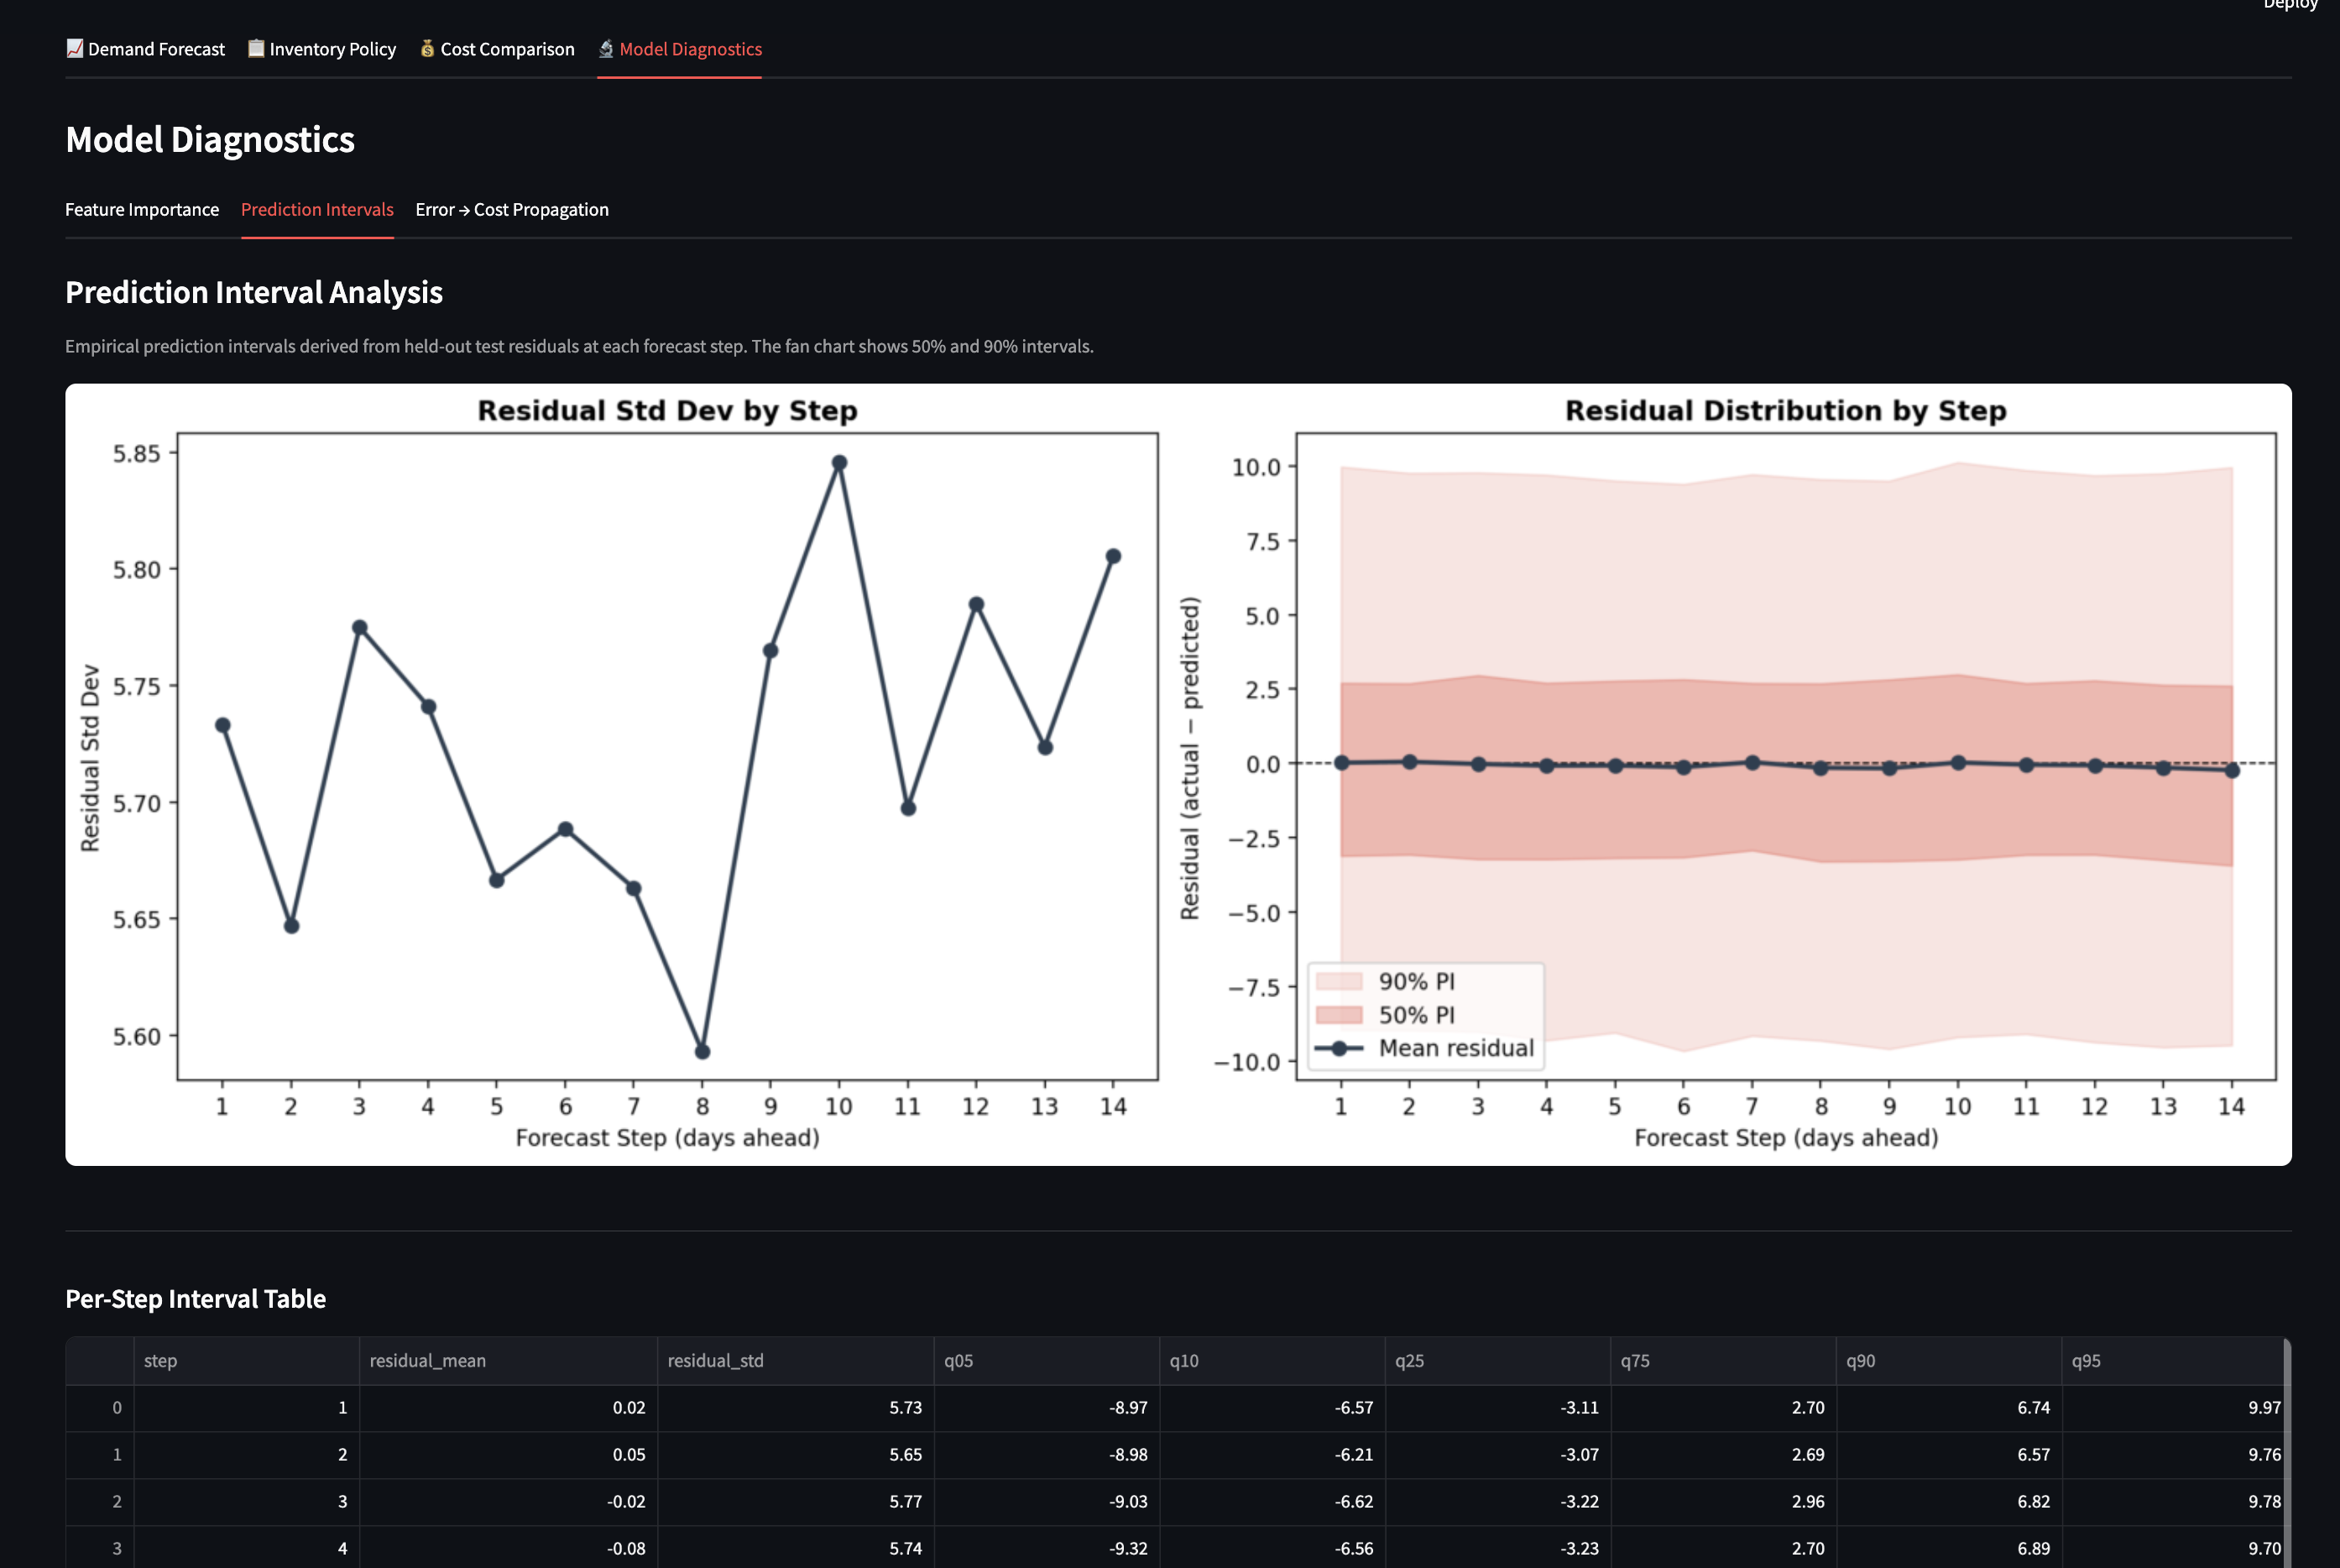
\includegraphics[width=\textwidth]{screenshots/diagnostics_prediction_intervals.png}
\caption{Prediction Intervals sub-tab. Left: residual standard deviation
by forecast step (1--14). Right: residual distribution fan chart with
50\% and 90\% confidence bands. Per-step interval table below.}
\label{fig:ss-pi}
\end{figure}

\begin{figure}[H]
\centering
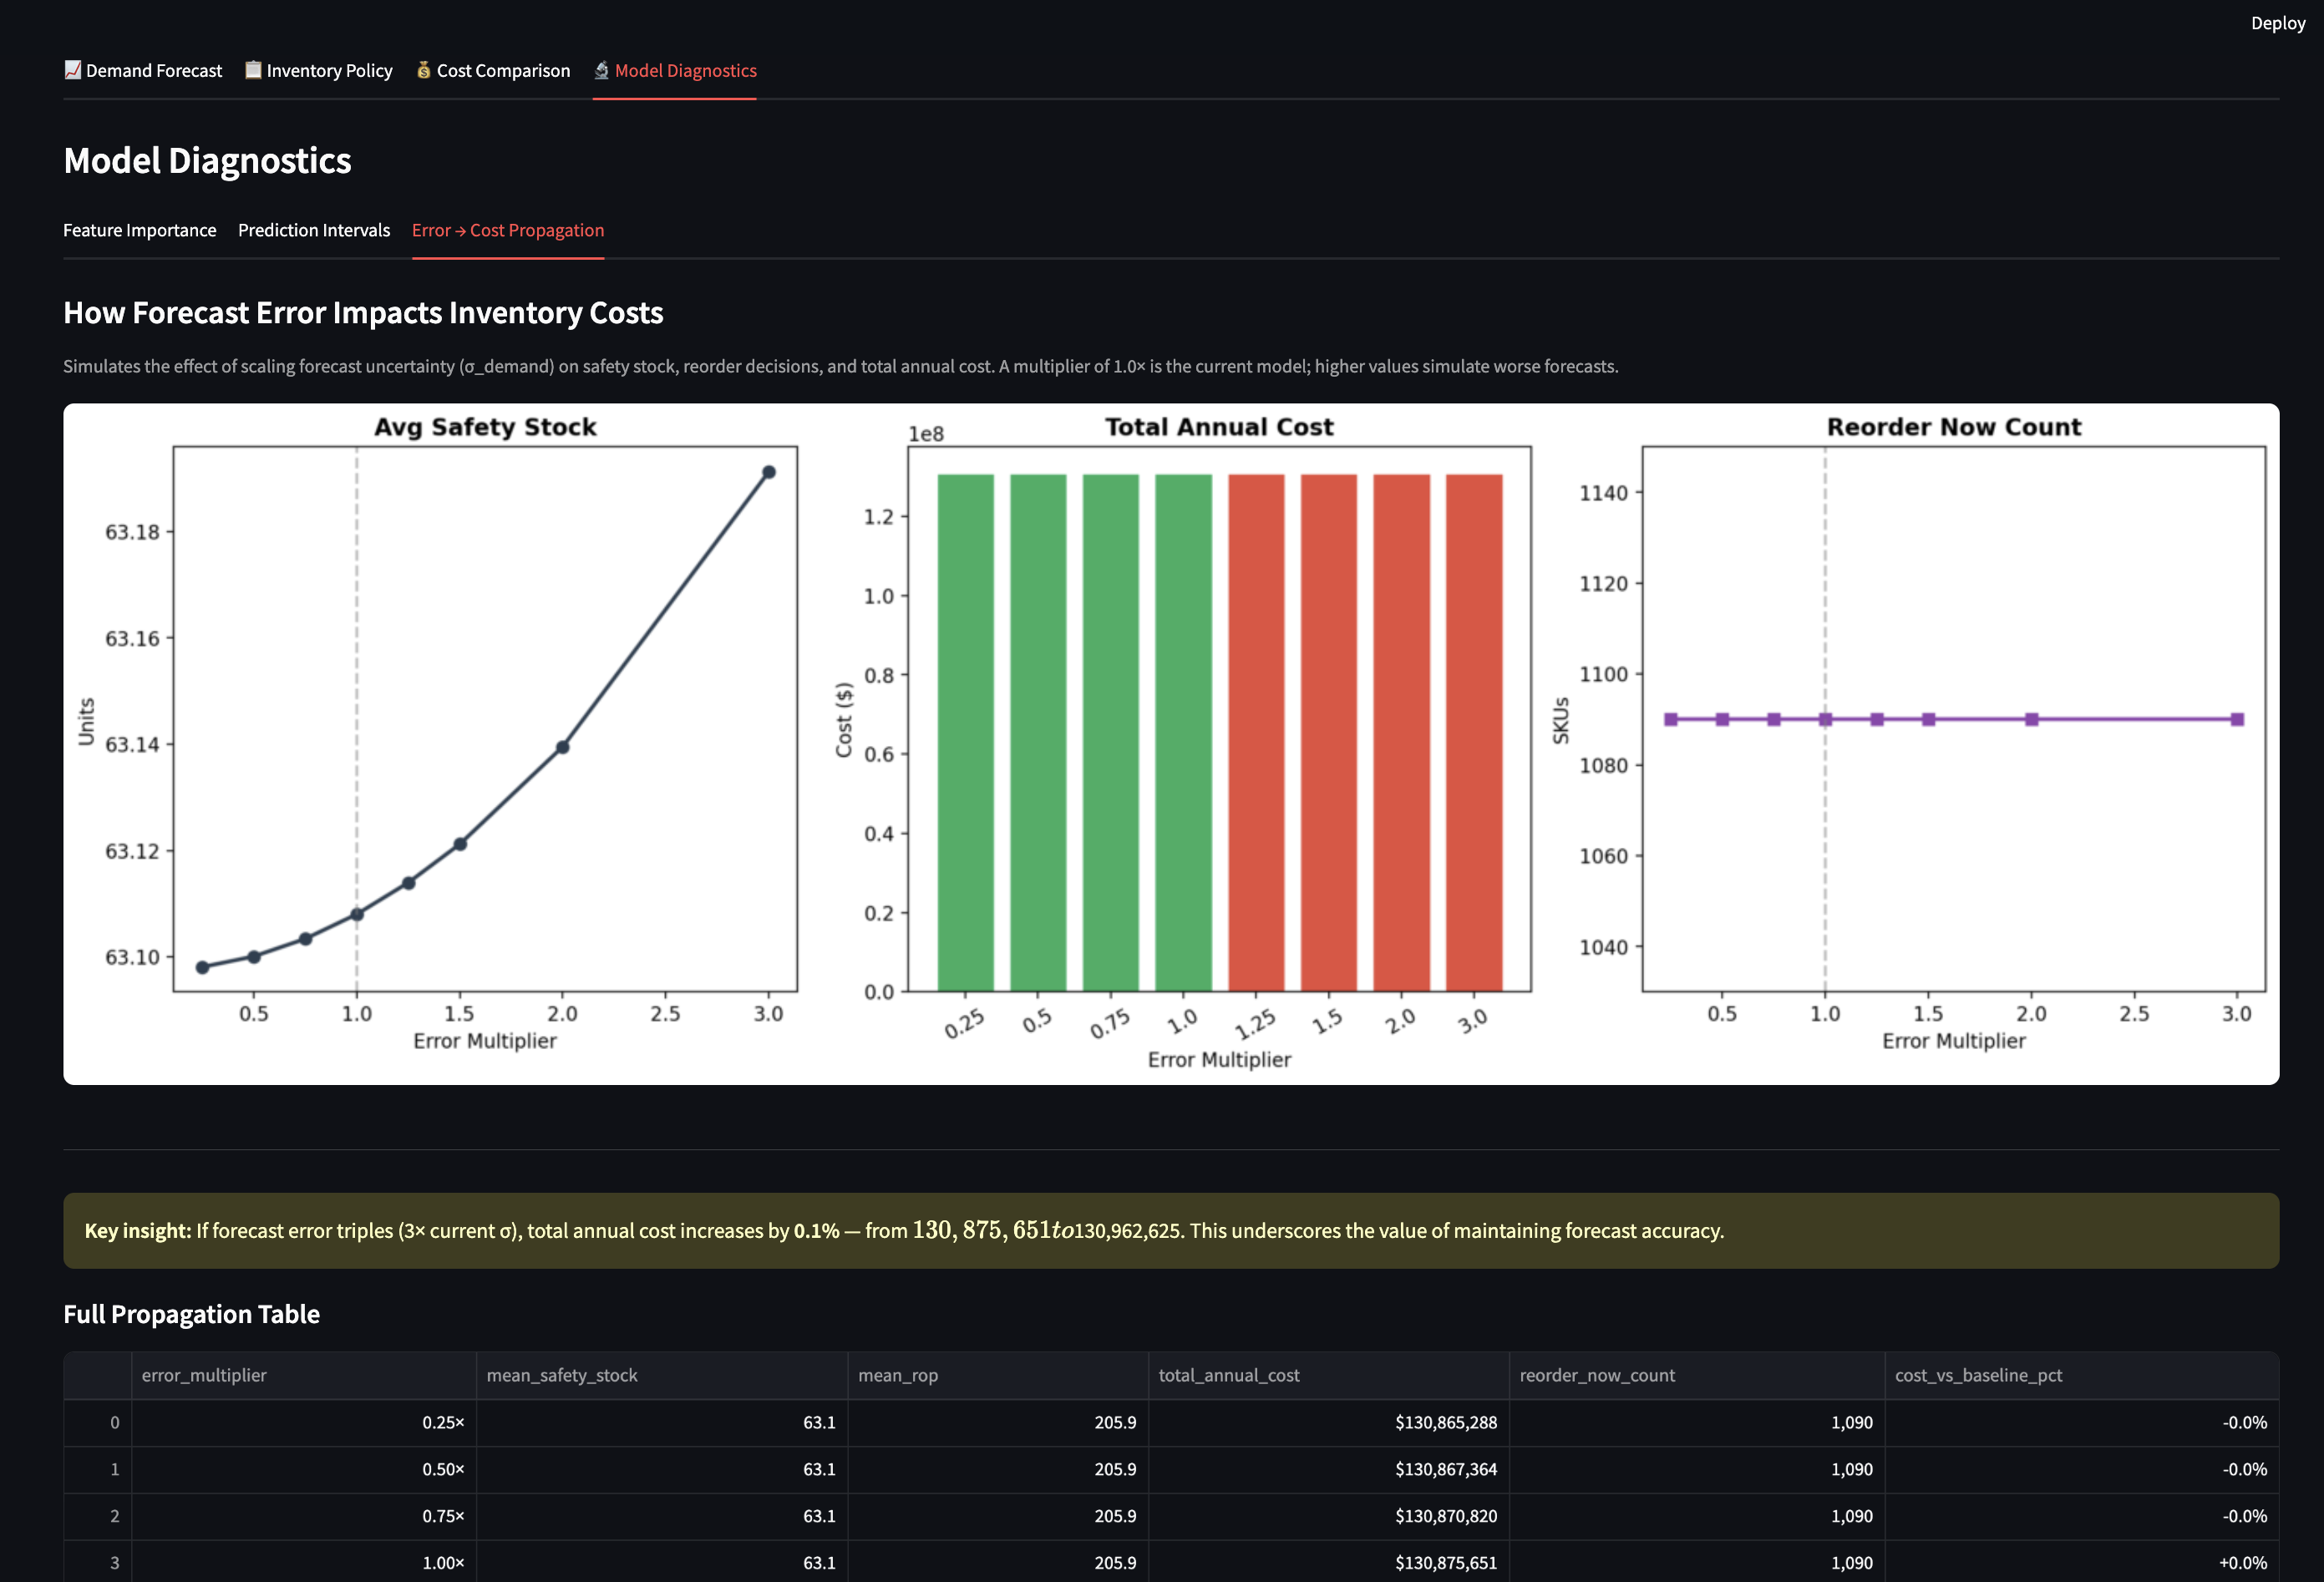
\includegraphics[width=\textwidth]{screenshots/diagnostics_error_cost.png}
\caption{Error-to-Cost Propagation sub-tab. Three-panel sensitivity
analysis: safety stock vs.\ error multiplier (left), total annual cost
(centre), and reorder count (right). The alert box quantifies worst-case
cost increase if forecast error triples.}
\label{fig:ss-error-cost}
\end{figure}

\end{document}
